% roomscan — English manuscript (IEEE conference format).
% Translated from paper/draft/00–09 (Thai) on 2026-09-17; re-framed around R3 vs pretrained (ADR-014) on 2026-09-25.
% Numbers from experiments/results/*/table.md via scripts/paper_numbers.py -> numbers.tex.
% Build:  make paper   (tectonic)   or   pdflatex main && bibtex main && pdflatex main && pdflatex main
\documentclass[conference]{IEEEtran}
\IEEEoverridecommandlockouts

\usepackage[T1]{fontenc}
\usepackage[utf8]{inputenc}
\usepackage{amsmath,amssymb}
\usepackage{booktabs}
\usepackage{graphicx}
\usepackage{multirow}
\usepackage{adjustbox}
\usepackage{tabularx}
\usepackage{url}
\urlstyle{tt}
\usepackage{xcolor}
\usepackage{siunitx}
\usepackage[hidelinks]{hyperref}
\usepackage{cite}

\graphicspath{{../figures/}}
\sisetup{detect-all,range-phrase=--,range-units=single,separate-uncertainty=true,multi-part-units=single}
\newcommand{\code}[1]{\texttt{#1}}
\sloppy   % long code identifiers in prose: prefer loose lines over overfull boxes
\newcommand{\fscore}{F@\SI{5}{cm}}

\begin{document}

\title{Teaching Monocular Depth the Metre with the Phone's Own LiDAR:\\
Fine-Tuned vs.\ Pretrained Depth Anything~V2 for Room Reconstruction, Measured Against a Laser Scanner}

% TODO: fill in author name(s) and affiliation before submission
\author{\IEEEauthorblockN{Author Name}
\IEEEauthorblockA{Affiliation\\
email@example.com}}

\maketitle

% generated by scripts/paper_numbers.py — do not edit

\newcommand{\rsGTCM}{2.1}
\newcommand{\rsGTSD}{0.5}
\newcommand{\rsGTF}{0.97}
\newcommand{\rsGTABSREL}{0.000}
\newcommand{\rsGTACC}{1.3}
\newcommand{\rsGTCOMP}{2.8}
\newcommand{\rsGTFtwo}{0.86}
\newcommand{\rsGTRtwo}{0.84}
\newcommand{\rsGTFfive}{0.97}
\newcommand{\rsGTRfive}{0.96}
\newcommand{\rsGTFten}{0.99}
\newcommand{\rsGTRten}{0.98}
\newcommand{\rsLIDARCM}{3.0}
\newcommand{\rsLIDARSD}{0.6}
\newcommand{\rsLIDARF}{0.93}
\newcommand{\rsLIDARABSREL}{0.018}
\newcommand{\rsLIDARACC}{2.2}
\newcommand{\rsLIDARCOMP}{3.9}
\newcommand{\rsLIDARFtwo}{0.54}
\newcommand{\rsLIDARRtwo}{0.52}
\newcommand{\rsLIDARFfive}{0.93}
\newcommand{\rsLIDARRfive}{0.91}
\newcommand{\rsLIDARFten}{0.98}
\newcommand{\rsLIDARRten}{0.97}
\newcommand{\rsORACLECM}{5.3}
\newcommand{\rsORACLESD}{1.3}
\newcommand{\rsORACLEF}{0.79}
\newcommand{\rsORACLEABSREL}{0.032}
\newcommand{\rsORACLEACC}{5.9}
\newcommand{\rsORACLECOMP}{4.7}
\newcommand{\rsORACLEFtwo}{0.46}
\newcommand{\rsORACLERtwo}{0.47}
\newcommand{\rsORACLEFfive}{0.79}
\newcommand{\rsORACLERfive}{0.82}
\newcommand{\rsORACLEFten}{0.90}
\newcommand{\rsORACLERten}{0.93}
\newcommand{\rsSPARSECM}{6.0}
\newcommand{\rsSPARSESD}{1.7}
\newcommand{\rsSPARSEF}{0.74}
\newcommand{\rsSPARSEABSREL}{0.036}
\newcommand{\rsSPARSEACC}{6.4}
\newcommand{\rsSPARSECOMP}{5.5}
\newcommand{\rsSPARSEFtwo}{0.38}
\newcommand{\rsSPARSERtwo}{0.39}
\newcommand{\rsSPARSEFfive}{0.74}
\newcommand{\rsSPARSERfive}{0.77}
\newcommand{\rsSPARSEFten}{0.88}
\newcommand{\rsSPARSERten}{0.91}
\newcommand{\rsSCENECM}{22.9}
\newcommand{\rsSCENESD}{2.1}
\newcommand{\rsSCENEF}{0.23}
\newcommand{\rsSCENEABSREL}{0.237}
\newcommand{\rsSCENEACC}{24.2}
\newcommand{\rsSCENECOMP}{21.6}
\newcommand{\rsSCENEFtwo}{0.08}
\newcommand{\rsSCENERtwo}{0.09}
\newcommand{\rsSCENEFfive}{0.23}
\newcommand{\rsSCENERfive}{0.27}
\newcommand{\rsSCENEFten}{0.41}
\newcommand{\rsSCENERten}{0.47}
\newcommand{\rsMETRICCM}{54.3}
\newcommand{\rsMETRICSD}{10.6}
\newcommand{\rsMETRICF}{0.03}
\newcommand{\rsMETRICABSREL}{0.382}
\newcommand{\rsMETRICACC}{70.3}
\newcommand{\rsMETRICCOMP}{38.3}
\newcommand{\rsMETRICFtwo}{0.01}
\newcommand{\rsMETRICRtwo}{0.01}
\newcommand{\rsMETRICFfive}{0.03}
\newcommand{\rsMETRICRfive}{0.04}
\newcommand{\rsMETRICFten}{0.06}
\newcommand{\rsMETRICRten}{0.10}
\newcommand{\rsGTa}{1.8}
\newcommand{\rsGTb}{1.2}
\newcommand{\rsGTc}{1.9}
\newcommand{\rsGTd}{2.8}
\newcommand{\rsGTe}{2.4}
\newcommand{\rsGTf}{2.3}
\newcommand{\rsLIDARa}{2.8}
\newcommand{\rsLIDARb}{2.4}
\newcommand{\rsLIDARc}{2.9}
\newcommand{\rsLIDARd}{4.1}
\newcommand{\rsLIDARe}{3.1}
\newcommand{\rsLIDARf}{3.0}
\newcommand{\rsORACLEa}{3.8}
\newcommand{\rsORACLEb}{6.2}
\newcommand{\rsORACLEc}{4.8}
\newcommand{\rsORACLEd}{7.5}
\newcommand{\rsORACLEe}{5.2}
\newcommand{\rsORACLEf}{4.5}
\newcommand{\rsSPARSEa}{4.5}
\newcommand{\rsSPARSEb}{6.1}
\newcommand{\rsSPARSEc}{5.5}
\newcommand{\rsSPARSEd}{9.1}
\newcommand{\rsSPARSEe}{5.9}
\newcommand{\rsSPARSEf}{4.6}
\newcommand{\rsSCENEa}{24.1}
\newcommand{\rsSCENEb}{26.0}
\newcommand{\rsSCENEc}{19.9}
\newcommand{\rsSCENEd}{23.2}
\newcommand{\rsSCENEe}{21.4}
\newcommand{\rsSCENEf}{23.1}
\newcommand{\rsMETRICa}{48.5}
\newcommand{\rsMETRICb}{61.6}
\newcommand{\rsMETRICc}{41.5}
\newcommand{\rsMETRICd}{48.9}
\newcommand{\rsMETRICe}{54.1}
\newcommand{\rsMETRICf}{71.0}
\newcommand{\rsFTFAROa}{10.8}
\newcommand{\rsFTFAROb}{13.8}
\newcommand{\rsFTFAROc}{17.6}
\newcommand{\rsFTFAROd}{21.1}
\newcommand{\rsFTFAROe}{12.4}
\newcommand{\rsFTFAROf}{11.9}
\newcommand{\rsFTLIDARa}{13.9}
\newcommand{\rsFTLIDARb}{19.0}
\newcommand{\rsFTLIDARc}{12.8}
\newcommand{\rsFTLIDARd}{12.5}
\newcommand{\rsFTLIDARe}{16.6}
\newcommand{\rsFTLIDARf}{24.6}
\newcommand{\rsFTLIDARALLa}{12.8}
\newcommand{\rsFTLIDARALLb}{16.7}
\newcommand{\rsFTLIDARALLc}{17.3}
\newcommand{\rsFTLIDARALLd}{12.2}
\newcommand{\rsFTLIDARALLe}{12.4}
\newcommand{\rsFTLIDARALLf}{22.5}
\newcommand{\rsSPARSEGAP}{0.6}
\newcommand{\rsSPARSEGAPLIDAR}{2.9}
\newcommand{\rsSPARSEVSSCENE}{3.8}
\newcommand{\rsLIDARGAPGTCM}{0.98}
\newcommand{\rsLIDARGAPGTSD}{0.25}
\newcommand{\rsORACLEGAPLIDARCM}{2.29}
\newcommand{\rsORACLEGAPLIDARSD}{1.11}
\newcommand{\rsCONFONECM}{3.07}
\newcommand{\rsCONFONEF}{0.93}
\newcommand{\rsCONFONEACC}{2.17}
\newcommand{\rsCONFONECOMP}{3.98}
\newcommand{\rsCONFTWOCM}{3.66}
\newcommand{\rsCONFTWOF}{0.93}
\newcommand{\rsCONFTWOACC}{2.08}
\newcommand{\rsCONFTWOCOMP}{5.23}
\newcommand{\rsWZOTCM}{3.07}
\newcommand{\rsWZOTF}{0.93}
\newcommand{\rsWZOTACC}{2.17}
\newcommand{\rsWZOTCOMP}{3.98}
\newcommand{\rsWOTFCM}{3.04}
\newcommand{\rsWOTFF}{0.93}
\newcommand{\rsWOTFACC}{2.23}
\newcommand{\rsWOTFCOMP}{3.85}
\newcommand{\rsFTFAROCM}{14.6}
\newcommand{\rsFTFAROSD}{4.0}
\newcommand{\rsFTFAROF}{0.31}
\newcommand{\rsFTFAROABSREL}{0.136}
\newcommand{\rsFTFARODELTAONE}{0.780}
\newcommand{\rsFTFARORtwo}{0.12}
\newcommand{\rsFTFARORfive}{0.34}
\newcommand{\rsFTFARORten}{0.57}
\newcommand{\rsFTLIDARCM}{16.6}
\newcommand{\rsFTLIDARSD}{4.7}
\newcommand{\rsFTLIDARF}{0.23}
\newcommand{\rsFTLIDARABSREL}{0.136}
\newcommand{\rsFTLIDARDELTAONE}{0.848}
\newcommand{\rsFTLIDARRtwo}{0.09}
\newcommand{\rsFTLIDARRfive}{0.26}
\newcommand{\rsFTLIDARRten}{0.49}
\newcommand{\rsFTLIDARALLCM}{15.7}
\newcommand{\rsFTLIDARALLSD}{4.0}
\newcommand{\rsFTLIDARALLF}{0.24}
\newcommand{\rsFTLIDARALLABSREL}{0.134}
\newcommand{\rsFTLIDARALLDELTAONE}{0.812}
\newcommand{\rsFTLIDARALLRtwo}{0.09}
\newcommand{\rsFTLIDARALLRfive}{0.28}
\newcommand{\rsFTLIDARALLRten}{0.51}
\newcommand{\rsFTTEACHERRATIO}{1.13}
\newcommand{\rsFTGAIN}{3.3}
\newcommand{\rsFTGAPORACLE}{11.2}
\newcommand{\rsDALARGECM}{6.45}
\newcommand{\rsDALARGESD}{2.42}
\newcommand{\rsDALARGEF}{0.74}
\newcommand{\rsDALARGEABSREL}{0.040}
\newcommand{\rsDALARGEDELTAONE}{0.979}
\newcommand{\rsDALARGESCAN}{355}
\newcommand{\rsDASMALLCM}{9.22}
\newcommand{\rsDASMALLSD}{3.48}
\newcommand{\rsDASMALLF}{0.64}
\newcommand{\rsDASMALLABSREL}{0.054}
\newcommand{\rsDASMALLDELTAONE}{0.964}
\newcommand{\rsDASMALLSCAN}{56}
\newcommand{\rsMIDASCM}{14.95}
\newcommand{\rsMIDASSD}{1.87}
\newcommand{\rsMIDASF}{0.35}
\newcommand{\rsMIDASABSREL}{0.110}
\newcommand{\rsMIDASDELTAONE}{0.873}
\newcommand{\rsMIDASSCAN}{18}
\newcommand{\rsSTRGTONECM}{2.1}
\newcommand{\rsSTRGTONEACC}{1.3}
\newcommand{\rsSTRGTONECOMP}{2.8}
\newcommand{\rsSTRGTONEF}{0.97}
\newcommand{\rsSTRGTONEABSREL}{0.000}
\newcommand{\rsSTRGTONEN}{391}
\newcommand{\rsSTRGTONESCAN}{2}
\newcommand{\rsSTRGTFIVECM}{4.4}
\newcommand{\rsSTRGTFIVEACC}{1.2}
\newcommand{\rsSTRGTFIVECOMP}{7.5}
\newcommand{\rsSTRGTFIVEF}{0.91}
\newcommand{\rsSTRGTFIVEABSREL}{0.000}
\newcommand{\rsSTRGTFIVEN}{78}
\newcommand{\rsSTRGTFIVESCAN}{1}
\newcommand{\rsSTRGTTENCM}{8.9}
\newcommand{\rsSTRGTTENACC}{1.2}
\newcommand{\rsSTRGTTENCOMP}{16.6}
\newcommand{\rsSTRGTTENF}{0.83}
\newcommand{\rsSTRGTTENABSREL}{0.000}
\newcommand{\rsSTRGTTENN}{40}
\newcommand{\rsSTRGTTENSCAN}{1}
\newcommand{\rsSTRGTTWENTYCM}{16.8}
\newcommand{\rsSTRGTTWENTYACC}{1.2}
\newcommand{\rsSTRGTTWENTYCOMP}{32.3}
\newcommand{\rsSTRGTTWENTYF}{0.68}
\newcommand{\rsSTRGTTWENTYABSREL}{0.000}
\newcommand{\rsSTRGTTWENTYN}{20}
\newcommand{\rsSTRGTTWENTYSCAN}{1}
\newcommand{\rsSTRORACLEONECM}{6.5}
\newcommand{\rsSTRORACLEONEACC}{7.1}
\newcommand{\rsSTRORACLEONECOMP}{5.8}
\newcommand{\rsSTRORACLEONEF}{0.74}
\newcommand{\rsSTRORACLEONEABSREL}{0.040}
\newcommand{\rsSTRORACLEONEN}{391}
\newcommand{\rsSTRORACLEONESCAN}{358}
\newcommand{\rsSTRORACLEFIVECM}{8.2}
\newcommand{\rsSTRORACLEFIVEACC}{5.6}
\newcommand{\rsSTRORACLEFIVECOMP}{10.9}
\newcommand{\rsSTRORACLEFIVEF}{0.72}
\newcommand{\rsSTRORACLEFIVEABSREL}{0.040}
\newcommand{\rsSTRORACLEFIVEN}{78}
\newcommand{\rsSTRORACLEFIVESCAN}{72}
\newcommand{\rsSTRORACLETENCM}{12.7}
\newcommand{\rsSTRORACLETENACC}{5.0}
\newcommand{\rsSTRORACLETENCOMP}{20.3}
\newcommand{\rsSTRORACLETENF}{0.65}
\newcommand{\rsSTRORACLETENABSREL}{0.041}
\newcommand{\rsSTRORACLETENN}{40}
\newcommand{\rsSTRORACLETENSCAN}{36}
\newcommand{\rsSTRORACLETWENTYCM}{20.9}
\newcommand{\rsSTRORACLETWENTYACC}{5.1}
\newcommand{\rsSTRORACLETWENTYCOMP}{36.7}
\newcommand{\rsSTRORACLETWENTYF}{0.52}
\newcommand{\rsSTRORACLETWENTYABSREL}{0.040}
\newcommand{\rsSTRORACLETWENTYN}{20}
\newcommand{\rsSTRORACLETWENTYSCAN}{19}
\newcommand{\rsSTRSCENEONECM}{22.7}
\newcommand{\rsSTRSCENEONEACC}{23.8}
\newcommand{\rsSTRSCENEONECOMP}{21.7}
\newcommand{\rsSTRSCENEONEF}{0.22}
\newcommand{\rsSTRSCENEONEABSREL}{0.240}
\newcommand{\rsSTRSCENEONEN}{391}
\newcommand{\rsSTRSCENEONESCAN}{346}
\newcommand{\rsSTRSCENEFIVECM}{22.7}
\newcommand{\rsSTRSCENEFIVEACC}{20.2}
\newcommand{\rsSTRSCENEFIVECOMP}{25.2}
\newcommand{\rsSTRSCENEFIVEF}{0.23}
\newcommand{\rsSTRSCENEFIVEABSREL}{0.236}
\newcommand{\rsSTRSCENEFIVEN}{78}
\newcommand{\rsSTRSCENEFIVESCAN}{71}
\newcommand{\rsSTRSCENETENCM}{25.0}
\newcommand{\rsSTRSCENETENACC}{18.9}
\newcommand{\rsSTRSCENETENCOMP}{31.0}
\newcommand{\rsSTRSCENETENF}{0.20}
\newcommand{\rsSTRSCENETENABSREL}{0.247}
\newcommand{\rsSTRSCENETENN}{40}
\newcommand{\rsSTRSCENETENSCAN}{36}
\newcommand{\rsSTRSCENETWENTYCM}{34.5}
\newcommand{\rsSTRSCENETWENTYACC}{21.4}
\newcommand{\rsSTRSCENETWENTYCOMP}{47.6}
\newcommand{\rsSTRSCENETWENTYF}{0.14}
\newcommand{\rsSTRSCENETWENTYABSREL}{0.268}
\newcommand{\rsSTRSCENETWENTYN}{20}
\newcommand{\rsSTRSCENETWENTYSCAN}{19}

\begin{abstract}
Reconstructing a room in 3D from a phone currently depends on a LiDAR sensor that only a minority of devices carry.
Monocular depth models have improved dramatically on single images, but there is no published number for how many
centimetres a room drifts when such a model replaces LiDAR inside an otherwise unchanged reconstruction pipeline.
This system-development paper builds a classical pipeline---per-frame depth $\rightarrow$ scale alignment
$\rightarrow$ TSDF fusion $\rightarrow$ mesh---in which \emph{the depth source and the scale-recovery strategy are
interfaces switched from a config file}, and measures mesh geometry against a laser-scanner reference on six real
rooms from ARKitScenes (2{,}352 frames) under identical conditions.
Results: the pipeline itself loses \SI{2.1 \pm 0.5}{cm} (Chamfer, \SI{4}{cm} voxels); iPad~Pro LiDAR adds only
\SI{1.0 \pm 0.3}{cm} (\fscore{} 0.93); Depth Anything~V2 with the correct scale on every frame loses
\SI{6.5 \pm 2.4}{cm} (\fscore{} 0.74), \SI{3.4}{cm} behind LiDAR.
With scale calibrated only once per room the error jumps to \SI{22.7 \pm 2.6}{cm} (\fscore{} 0.22), and an
uncalibrated ``metric'' model gives \SI{49}{cm}. Per-frame analysis shows the cause: the model's scale swings by
several times with the content of each view, not with time.
Fitting scale per frame on only $\sim$200 sparse metric points---the kind a phone's visual-inertial tracker
provides for free---recovers \SI{\rsSPARSECM}{cm} (\fscore{} \rsSPARSEF), essentially the oracle.
Model size (Large$\rightarrow$Small) costs just \SI{2.8}{cm} for a $7\times$ speed-up, and frame rate governs
coverage rather than accuracy ($\geq 0.8$~fps is needed).
The product conclusion is that the gap between devices with and without LiDAR is a per-frame scale problem, solvable
with metric data from VIO rather than with a larger model. Code, every experiment config, and every run's metrics are released.
\end{abstract}


\begin{IEEEkeywords}
monocular depth estimation, transfer learning, metric depth, LiDAR supervision, TSDF fusion, 3D room reconstruction, ARKitScenes
\end{IEEEkeywords}

\section{Introduction and Business Motivation}

\subsection{Problem}
Scanning a room into a 3D model is already a consumer feature on iPhone~Pro and iPad~Pro through Apple RoomPlan and
apps such as Polycam, all of which rely on the \emph{LiDAR sensor} for directly metric depth. Devices with LiDAR are,
however, a minority of the market: non-Pro iPhones and almost every Android phone have none. The alternative for these
devices is \emph{monocular depth estimation}---networks that predict depth from a single RGB image---which advanced
rapidly between 2020 and 2024 (MiDaS, Depth Anything) to the point of producing visually convincing results on single images.

The question a product team must answer before investing is: \textbf{if LiDAR is replaced by a monocular model while the
rest of the system stays the same, by how many centimetres is the reconstructed room wrong, and which use cases does that
still serve} (floor-area estimation, furniture placement, renovation measurement)? Monocular-depth research reports
per-image metrics (AbsRel, $\delta_1$) on benchmarks, which do not translate into ``how crooked is the wall.''
End-to-end reconstruction systems (Atlas, NeuralRecon, SimpleRecon) design their whole pipeline around their own model,
so the \emph{depth source} cannot be compared in isolation.

Some recent models claim to output \emph{metres} directly, without calibration (DA-v2 Metric-Indoor, ZoeDepth, Depth
Pro)---if that held, the question above would reduce to choosing a model. These models, however, are trained on data
that are not a phone's camera (DA-v2 Metric-Indoor on rendered Hypersim images), and inside a real room-reconstruction
pipeline the room comes out \SI{\rsMETRICCM}{cm} wrong (\S\ref{sec:exp1}). The direct remedy is \emph{transfer
learning}: keep training the model on depth from the target domain. The question is where those labels come from---the
\$20k laser scanner used to build research datasets, or the \emph{LiDAR already inside Pro phones}, which an app maker
can collect at scale. If the latter works, the minority of devices with LiDAR can be the teacher of the majority
without it.

\subsection{Research question}
\textbf{Main question:} is DA-v2 Metric-Indoor fine-tuned with depth from the iPad's LiDAR (no laser scanner at
training time) \emph{better than the same model pretrained}, when measured against the Faro laser scanner---the raw
ground truth ARKitScenes ships---both as a room mesh (centimetres on the wall) and as per-frame depth, on rooms never
used for training?
\textbf{Supporting questions:} (a) how much better is a laser teacher than a phone-LiDAR teacher; (b) where does the
fine-tuned model stand relative to using a sensor at run time (LiDAR, sparse points per frame); (c) where does the
remaining error come from?

\subsection{Approach}
This is a \emph{system-development} study. We build a classical room-reconstruction pipeline (per-frame depth
$\rightarrow$ scale alignment $\rightarrow$ TSDF voxel fusion $\rightarrow$ mesh) in which \textbf{the depth source is
the single swappable variable}, so ``pretrained'' and ``fine-tuned'' are two rows that differ only in a checkpoint
name, and every other depth source can be priced through the same pipeline as context:

\begin{table*}[t]
\centering\small
\begin{tabularx}{\textwidth}{@{}lX@{}}
\toprule
Depth source & Stands for \\
\midrule
\textbf{DA-v2 Metric-Indoor pretrained / fine-tuned with a LiDAR teacher (R3)} & \textbf{main question: a device with no sensor and no calibration} \\
Faro laser (\code{highres\_depth}) & upper bound of the pipeline: its own loss with perfect depth \\
ARKit LiDAR (\code{lowres\_depth}, $256\times192$) & what iPhone~Pro does today (and R3's teacher) \\
Monocular (Depth Anything V2, MiDaS) $\times$ scale strategy & ceiling and cost of supplying scale at run time instead of training \\
\bottomrule
\end{tabularx}
\end{table*}

Fine-tuning uses ARKitScenes rooms disjoint from the test rooms at the \code{visit\_id} level and trains only the DPT
neck and metric head. Evaluation uses Faro twice: a reference mesh fused from Faro depth on six test rooms (3D), and Faro
depth per frame directly on those rooms and on \rsVN{} more from the Validation fold (2D). Isolating \emph{ScaleAligner}
as a separate stage further lets us separate ``wrong shape'' from ``wrong scale'': \code{oracle\_frame} (fit per frame
against GT) is a model's ceiling, \code{per\_scene} is a one-off calibration, and \code{sparse\_points} (fit per frame
on a few hundred metric points) is what a system with a VIO tracker can do.

\subsection{Main results}
\begin{itemize}
\item \textbf{The LiDAR-teacher fine-tune (R3) beats the pretrained model in every test room:} Chamfer
\SI{\rsMETRICCM}{cm}$\rightarrow$\SI{\rsFTLIDARALLCM}{cm} ($\rsMAINGAIN\times$, \rsMAINWINS/\rsMAINN{} rooms), \fscore{}
\rsMETRICF$\rightarrow$\rsFTLIDARALLF, per-frame AbsRel against Faro \rsMETRICSIXABSREL$\rightarrow$\rsFTLIDARALLABSREL{}
---with no calibration and no sensor at run time (\S\ref{sec:main}).
\item \textbf{The same holds on \rsVN{} rooms that took part in nothing:} AbsRel \rsVMETRICABSREL$\rightarrow$\rsVFTALLABSREL,
better in \rsVWINS/\rsVN{} rooms (exact Wilcoxon $p=\rsVP$) (\S\ref{sec:main}).
\item \textbf{A laser teacher is not measurably better than a phone-LiDAR teacher:} \SI{\rsFTFAROCM}{cm} (Faro) /
\SI{\rsFTLIDARCM}{cm} (LiDAR, 10 rooms) / \SI{\rsFTLIDARALLCM}{cm} (LiDAR, 24 rooms), within the across-room std
(\S\ref{sec:finetune}).
\item An intrinsics-conditioned metric model (Depth Pro), given the real focal length and no fine-tuning, reaches only
\SI{\rsDEPTHPROCM}{cm}---knowing the camera does not replace in-domain labels (\S\ref{sec:finetune}).
\item \textbf{R3 does not reach a sensor:} the pipeline itself loses \SI{\rsGTCM \pm \rsGTSD}{cm}, iPad LiDAR
\SI{\rsLIDARCM \pm \rsLIDARSD}{cm}, monocular depth with the correct scale on every frame
\SI{\rsORACLECM \pm \rsORACLESD}{cm}, and a per-frame fit on $\sim$200 sparse points (VIO proxy) \SI{\rsSPARSECM}{cm}
(\S\ref{sec:exp1}).
\item \textbf{The remaining error is scale that swings per view, not shape:} one calibration per room gives
\SI{\rsSCENECM \pm \rsSCENESD}{cm} uniformly; the model's scale varies several-fold within one scan with the content of
the frame, not with time (\S\ref{sec:discussion}). Fine-tuning removes the domain bias; the per-frame factor still has
to come from metric data at run time.
\item A $13\times$ smaller model (DA-v2 Small) costs \SI{1.0}{cm} for a $6\times$ speed-up, and frame count governs
coverage, not accuracy ($\geq 0.8$~fps is needed).
\end{itemize}

\subsection{Contributions}
\begin{enumerate}
\item \textbf{A measured answer to ``does fine-tuning on a phone's own LiDAR really help a metric monocular model?''},
against a laser scanner on held-out rooms in 3D (6 rooms) and 2D (6 $+$ \rsVN{} rooms), with the checkpoints, the room
split and the room-selection scripts released (\S\ref{sec:ftsetup}, \S\ref{sec:main}).
\item A teacher ablation (Faro vs.\ LiDAR, 10 vs.\ 24 rooms) and an intrinsics-conditioned baseline under one training
recipe (\S\ref{sec:finetune}).
\item An open-source pipeline in which \code{DepthSource} and \code{ScaleAligner} are interfaces switched from config
without touching the orchestrator, so every table is ``one loop, one variable'' and a newly trained checkpoint becomes
a new row immediately (\S\ref{sec:design}).
\item ``Centimetres on the wall'' for Faro / LiDAR / monocular $\times$ scale strategy through one pipeline, and an
analysis showing that monocular error comes from per-view scale, not temporal drift---which explains both why
fine-tuning helps and why it is not enough (\S\ref{sec:exp1}, \S\ref{sec:discussion}).
\item Per-scan cost (time, frames, model size, LiDAR confidence weighting) for business decisions (\S\ref{sec:business}).
\end{enumerate}

\paragraph{What this paper does \emph{not} claim}
It does not claim to beat Atlas / NeuralRecon / SimpleRecon---they are not compared, and this pipeline is not designed to
compete. It does not claim that fine-tuning makes LiDAR unnecessary: R3 (\SI{\rsFTLIDARALLCM}{cm}) remains far from
LiDAR (\SI{\rsLIDARCM}{cm}) and from having metric points at run time (\SI{\rsSPARSECM}{cm}). It does not claim that a
LiDAR teacher equals or beats a laser teacher---R1 and R2 differ in both label and number of training views
(\S\ref{sec:ftsetup}) and by less than the across-room std. Only the head of one model is fine-tuned (frozen encoder,
ARKitScenes, iPad camera); every other model is used pretrained, and other phone cameras are not measured.

\section{Related Work}\label{sec:related}

\subsection{Monocular depth estimation}
Monocular depth models fall into two families according to what their output promises.

\paragraph{Relative / affine-invariant} MiDaS~\cite{midas} introduced training across many datasets with a loss that
ignores scale and shift, giving strong cross-domain generalisation at the price of an output that is \emph{disparity up
to an affine transform}: two constants $(s, t)$ per image must be known to obtain metres. Depth Anything~\cite{da1}
and Depth Anything~V2~\cite{da2} extend the idea with large unlabelled corpora and synthetic teachers, giving much sharper
edges and detail while remaining affine-invariant in disparity. We use DA-v2 (Large / Small) and MiDaS small as
representatives of this family and \textbf{treat $(s,t)$ as an experimental variable} (the \code{ScaleAligner}) rather
than hiding it in the model.

\paragraph{Metric} ZoeDepth~\cite{zoedepth} and the metric variants of DA-v2 (fine-tuned on Hypersim / Virtual KITTI)
aim to output metres directly. Metric3D~\cite{metric3d} identifies the camera focal length as the main ambiguity and
resolves it by normalising images to a canonical camera. These works report per-image AbsRel/$\delta_1$ on NYUv2/KITTI;
our results (\S\ref{sec:metric}) show that on real room video the per-frame scale of a metric model still swings from
$-60\%$ to $+80\%$ within one scan---invisible to per-image metrics, immediately visible once frames are fused into one
volume.

\paragraph{Conditioning on the camera, or on a teacher} Two families answer the scale ambiguity differently. One
conditions the network on camera intrinsics---Metric3D~\cite{metric3d}, UniDepth~\cite{unidepth}, and Depth
Pro~\cite{depthpro}, which estimates the focal length itself---so a metre prediction is tied to a known field of view.
The other adapts a pretrained model to the target domain with depth labels, which is what the metric DA-v2 variants do
on Hypersim. We take the second route but change where the labels come from: instead of a laser scanner or a synthetic
renderer, the teacher is the depth sensor already shipping in consumer phones. This puts a price on the teacher---the
question a product team actually faces---rather than on the architecture, and it is measured against a laser scanner
both in mesh centimetres on held-out rooms and in per-frame AbsRel on 26 rooms, not on a single-image benchmark
(\S\ref{sec:main}). The two families are complementary: an
intrinsics-conditioned model could be fine-tuned with the same LiDAR labels. We measure one of them
(Depth Pro, handed the camera's true focal length) as the Level-0 row of Exp.~6: on these captures it does
\emph{not} deliver usable metric depth (\S\ref{sec:finetune}), which is why fine-tuning is the axis we study.

\paragraph{Mobile LiDAR depth} ARKit provides $256\times192$ depth fusing LiDAR with imagery; ARKitScenes~\cite{arkitscenes}
is the first dataset to release both this depth and Faro laser-scanner depth for the same rooms, making a direct
``mobile LiDAR vs.\ laser'' comparison possible. We use both as two rows of the same table.

\subsection{Multi-view 3D reconstruction from video}
\paragraph{Classical depth fusion} Volumetric TSDF fusion~\cite{curless96} and KinectFusion~\cite{kinectfusion}
combine many depth frames through a truncated signed distance per voxel and extract the surface with marching cubes.
The property we need is that \textbf{fusion neither knows nor cares where depth comes from}---as long as it is metric
and posed---so it is a fair ``fixed part'' for every source. We use the Open3D implementation~\cite{open3d}.

\paragraph{End-to-end learned reconstruction} Atlas~\cite{atlas} regresses a TSDF directly from multi-image features,
NeuralRecon~\cite{neuralrecon} does so incrementally in real time, and SimpleRecon~\cite{simplerecon} shows that good
multi-view depth plus classical fusion is competitive. These are strong ScanNet baselines, but all learn depth
\emph{from multiple images}; they do not answer ``what room do you get from a per-image monocular model plus the
device's VIO pose,'' which is the situation of an app on a device without LiDAR. We therefore \textbf{do not compare
against this group} and make no claim of superiority.

\paragraph{Scale in monocular SLAM / reconstruction} Using monocular depth inside SLAM requires per-frame scale
recovery, e.g.\ from sparse tracked points (CNN-SLAM~\cite{cnnslam} and successors), or joint optimisation of
scale/shift with pose (MonoSDF~\cite{monosdf} uses monocular priors in a neural surface). Our \code{sparse\_points}
aligner follows this line; we evaluate it next to \code{oracle\_frame} and \code{per\_scene} so that the ``price of not
knowing scale'' is measured at three levels of available metric information.

\subsection{Room-scanning products}
Apple RoomPlan~\cite{roomplan} produces a floor plan and furniture boxes from LiDAR on iPhone/iPad~Pro; Polycam and
similar apps produce meshes or photogrammetry. All require LiDAR for room mode or fall back to slow offline
photogrammetry with many photos. No public report states how many centimetres these products deviate from a laser
scanner; this paper provides that number at least for our own pipeline.

\subsection{Position of this work}
\begin{table*}[t]
\centering\small
\begin{adjustbox}{max width=\textwidth}
\begin{tabular}{@{}lcccc@{}}
\toprule
 & Trains & Compares depth sources & Reference & Metrics \\
\midrule
Monocular depth papers & \checkmark & $\times$ (one model) & per-image depth & AbsRel, $\delta$ \\
Atlas / NeuralRecon / SimpleRecon & \checkmark & $\times$ (multi-view only) & ScanNet mesh & Chamfer, F-score \\
\textbf{This work} & head only (LiDAR teacher) & \checkmark\ laser / LiDAR / mono $\times$ aligner $\times$ teacher & Faro laser (ARKitScenes) & Chamfer, F@$\tau$, per-frame AbsRel/$\delta$, time \\
\bottomrule
\end{tabular}
\end{adjustbox}
\end{table*}

\section{System Design}\label{sec:design}

\subsection{Design principle: one pipeline, one variable}
The research question (``change only the depth source---how much changes?'') imposes three architectural requirements:
\begin{enumerate}
\item \textbf{Every depth source must pass through the same code after the point where it is produced}---no special
branch for mono or LiDAR in fusion or evaluation.
\item \textbf{Whatever can be swapped is swapped from config}, not by editing code: one result table $=$ one YAML file.
\item \textbf{The paper's code is the product's code}: the same system must accept ARCore depth or a smaller model on
the day an MVP ships, without a rewrite.
\end{enumerate}
Requirement~1 leads to the \code{DepthSource} interface; requirement~2 to a string$\rightarrow$class registry and
base-plus-override configs; requirement~3 to a single monolithic package with no service, database or experiment
tracker---appropriate for a one-person, ten-week project.

\subsection{Overview}
\begin{figure*}[t]
\centering
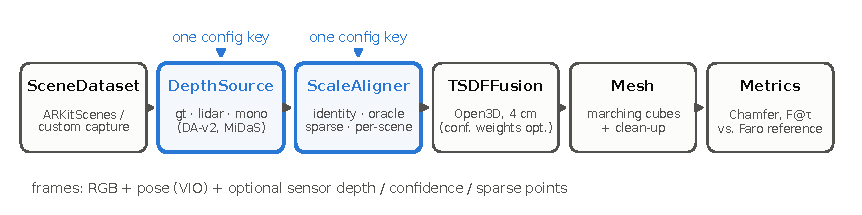
\includegraphics[width=\textwidth]{pipeline}
\caption{Pipeline components. The two highlighted boxes are the only things that change between rows of a result
table; everything to their right is fixed (Open3D \code{ScalableTSDFVolume}, marching cubes, cluster filtering).
Frame stride (Exp.~3) is a dataset parameter; voxel size (Exp.~2) is a fusion parameter.}
\label{fig:pipeline}
\end{figure*}

Fig.~\ref{fig:pipeline} shows the data flow. Per frame there are three typed hand-over points:
\begin{table*}[t]
\centering\small
\begin{adjustbox}{max width=\textwidth}
\begin{tabular}{@{}lll@{}}
\toprule
Point & Type & Owner \\
\midrule
\code{Frame\{rgb, pose\_c2w, gt\_depth?, extra\}} & from \code{SceneDataset} & dataset mapping \\
\code{pred: (H,W) float32}, relative \emph{or} metric & \code{DepthSource.get\_depth(frame)} & source declares \code{is\_metric} \\
\code{depth\_m: (H,W) float32} metres, $0=$ invalid & \code{ScaleAligner.align(pred, frame)} & invariant: metric after the aligner \\
\bottomrule
\end{tabular}
\end{adjustbox}
\end{table*}

Invariants enforced in code, not just documented: (i) values are metres after the aligner; (ii) \code{pose\_c2w} is
camera-to-world and is inverted in exactly one place (\code{TSDFFusion.integrate}); (iii) intrinsics are bound to a
resolution---resizing requires \code{Intrinsics.scaled()}; (iv) \code{is\_metric=True} $\Rightarrow$
\code{aligner=identity} and \code{is\_metric=False} $\Rightarrow$ \code{aligner$\neq$identity}---the pipeline fails at
construction if the pair is wrong.

\subsection{DepthSource: depth as a strategy}
{\small\begin{verbatim}
class DepthSource(ABC):
    name: str
    is_metric: bool
    def get_depth(self, frame) -> np.ndarray
        # (H,W) float32; 0/NaN = invalid
\end{verbatim}}
It takes the whole \code{Frame} rather than an RGB image because each source needs different inputs: \code{gt}
reads \code{frame.gt\_depth}, \code{lidar} reads \code{frame.extra["lidar\_depth"]} (plus confidence), \code{mono}
reads \code{frame.rgb}. One signature covers all cases without edits when \code{arcore} is added.
\code{MonocularDepth} does three things that belong neither to the model nor to the aligner: it rotates the image
upright according to \code{sky\_direction}, converts disparity to $1/x$ so that ``larger $=$ farther,'' and masks
invalid values. Models (\code{DepthModel}: DA-v2, MiDaS) form a second registry under \code{mono}, so Exp.~4 (model
size) is just \code{depth.model=\ldots}.

\subsection{ScaleAligner: scale as a separate stage}
A relative model gives depth up to an affine transform. \emph{How} $(s,t)$ is obtained is a \textbf{system decision}
that should be measured separately from the model, so it is its own stage:
\begin{table*}[t]
\centering\small
\begin{adjustbox}{max width=\textwidth}
\begin{tabular}{@{}lll@{}}
\toprule
Aligner & Fits $(s,t)$ & Meaning \\
\midrule
\code{identity} & --- & GT / LiDAR / metric models \\
\code{oracle\_frame} & per frame, against GT depth & model ceiling (not deployable) \\
\code{per\_scene} & once, on $N$ frames spread over the scan, then frozen & one-off calibration \\
\code{sparse\_points} & per frame, against $\sim$200 sparse metric points & the MVP path (VIO feature points) \\
\bottomrule
\end{tabular}
\end{adjustbox}
\end{table*}
The gap \code{oracle\_frame} $\rightarrow$ \code{per\_scene} is ``the price of not knowing scale''---an experimental
result, not noise; \code{sparse\_points} measures how much of that price a phone's tracker can pay back.

\paragraph{Fitting space} Affine-invariant models are affine in \emph{disparity}, not depth; fitting
$gt \approx s\cdot pred + t$ in depth space is the wrong model. We therefore fit $1/gt \approx s\cdot(1/pred) + t$
(least squares with three rounds of trimming the worst 20\% of residuals) and invert back. On scene 42444474 this
change alone moved mono$+$oracle from \SI{15.2}{cm} to \SI{5.4}{cm}---an example of why the aligner must be testable in
isolation.

\paragraph{Sparse points} ARKitScenes ships no ARKit feature points, so \code{sparse\_points} is evaluated against a
proxy: $N{=}200$ pixels sampled per frame (deterministically) from the LiDAR frame at confidence~2, which is what a
tracker hands the pipeline---a few hundred metric depths per frame, nothing dense. The fit is per frame in inverse
depth with two rounds of 10\% trimming; frames with fewer than 20 usable points reuse the previous frame's $(s,t)$,
as a deployed system would when tracking momentarily loses features. The proxy is optimistic in one respect (LiDAR
points are cleaner than triangulated VIO features) and pessimistic in another (VIO points cluster on texture, ours are
uniform); we treat the row as an \emph{upper bound of real VIO}.

\subsection{Fixed parts: fusion, post-processing, evaluation}
\begin{itemize}
\item \textbf{Fusion:} Open3D \code{ScalableTSDFVolume}, \SI{4}{cm} voxels, \code{sdf\_trunc}$=3\times$voxel,
depth \SIrange{0.1}{5}{m}; every source is resampled to $256\times192$ (the LiDAR resolution) before integration for
fairness, and only pixels where the reference has depth are integrated (\code{mask\_to\_gt})---no source is penalised
for seeing beyond the Faro coverage. An optional per-pixel integer weight from the sensor's confidence map
(\code{fusion.confidence\_weights}) is off for every main result and used only in Exp.~5.
\item \textbf{Post-processing:} small clusters removed; no decimation.
\item \textbf{Reference:} ARKitScenes provides no laser mesh; we fuse Faro \code{highres\_depth} from every frame at
\SI{1}{cm} voxels once per scene into \code{reference\_mesh.ply}. The \code{gt} row at \SI{4}{cm} therefore measures
``pipeline loss,'' not zero.
\item \textbf{3D metrics} (fixed protocol in \code{metrics\_3d.py}): 200k points sampled on both meshes (fixed seed);
accuracy $=$ mean pred$\rightarrow$ref distance, completeness $=$ ref$\rightarrow$pred, Chamfer $=$ their mean;
precision/recall/F-score at \SI{2}{}/\SI{5}{}/\SI{10}{cm} (\textbf{\fscore{} is the headline}); normal consistency
$=$ mean $|n_{pred}\cdot n_{ref}|$.
\item \textbf{2D metrics} per frame (RMSE, AbsRel, $\delta_{1\text{--}3}$) compare depth \emph{after} alignment with GT
depth, to tell whether error arises before or after fusion.
\end{itemize}

\subsection{Config, registry and experiments}
\code{configs/base.yaml} defines every value; \code{configs/experiments/expN.yaml} $=$ base $+$ a list of runs, each a
handful of dotted-key overrides. \code{roomscan sweep} runs every run $\times$ every scene and writes a resolved
\code{config.yaml} plus \code{metrics.json} per run; \code{roomscan report} aggregates them into \code{summary.csv}
and one \code{table.md} per experiment. The tables in \S\ref{sec:results} are copied from those files.

Every kind of extension is one new file plus one registry line, without touching \code{pipeline.py}: a depth source
(ARCore), a model (a compressed variant), an aligner, a dataset (a real room captured by the app;
\code{dataio/custom.py} reads the app's folder format), or an experiment. The rule that guards the design: if adding
something requires editing \code{pipeline.py}, stop and write an architecture decision record. Over the project this
happened exactly once (per-pixel confidence weights, two lines), and it is recorded as such.

\subsection{Deliberately not done}
GPU TSDF, an experiment tracker, and pose estimation (the dataset's ARKit VIO poses are used) are out of scope; a
minimal web service and viewer exist as a separate package importing the pipeline, and none of these affect the numbers.

\section{Experimental Setup}\label{sec:setup}

\subsection{Dataset: ARKitScenes}
We use ARKitScenes~\cite{arkitscenes} because it is the only dataset that provides \textbf{all three} things the
question needs for the same room: RGB video from a real device (iPad~Pro), depth from that device's LiDAR
(\code{lowres\_depth}, $256\times192$), and depth from a Faro laser scanner registered to the camera poses
(\code{highres\_depth}, $1920\times1440$). The ``iPhone~Pro today'' row and the reference therefore come from one scan,
with no cross-sensor alignment of our own.

\begin{table*}[t]
\centering\small
\begin{adjustbox}{max width=\textwidth}
\begin{tabular}{@{}lll@{}}
\toprule
Asset & Resolution / rate & Role \\
\midrule
\code{vga\_wide} RGB & $640\times480$, 30 fps & input to monocular models (rotated upright) \\
\code{lowres\_depth} $+$ \code{confidence} & $256\times192$, 60 fps & depth source \code{lidar}; sparse-point proxy; Exp.~5 weights \\
\code{highres\_depth} (Faro) & $1920\times1440$, \textbf{$\sim$2.7--4 fps} & depth source \code{gt} and \textbf{reference mesh} \\
\code{lowres\_wide.traj} & $\sim$10 Hz & pose (ARKit VIO), slerp/lerp-interpolated to each frame \\
\code{lowres\_wide\_intrinsics} & per frame & scan median, scaled to resolution \\
\bottomrule
\end{tabular}
\end{adjustbox}
\end{table*}

Two dataset constraints shape the experiments: (1) Faro depth exists only for the frames Apple kept ($\sim$3~fps), so
every source is evaluated \textbf{on this same frame set} and Exp.~3 (frame stride) measures coverage more than
compute (\S\ref{sec:stride}); (2) no laser mesh is provided, so we build one (\S\ref{sec:reference}).

\begin{table*}[t]
\centering\small
\caption{Scenes. Extent $=$ axis-aligned extent of the reference mesh (what Faro saw); Faro frames $=$ number of
frames every row is evaluated on. Total: 2{,}352 frames / \SI{577}{s} of video.}
\label{tab:scenes}
\begin{adjustbox}{max width=\textwidth}
\begin{tabular}{@{}lllrrl@{}}
\toprule
video\_id & Room (3DOD labels) & Extent (m) & Scan (s) & Faro frames & Role \\
\midrule
42444474 & open-plan kitchen/dining under sloped roof, glass table/rail, brick wall & $9.9\times5.1\times4.2$ & 88 & 236 & large $+$ glass (dev.\ scene) \\
47333774 & standard bedroom (bed, shelf, cabinet, table) & $5.1\times4.9\times3.3$ & 90 & 375 & standard \#1 \\
47115299 & large living room (4 tables, 2 sofas, TV) & $8.1\times6.1\times2.5$ & 91 & 324 & large \\
42897743 & bathroom (bathtub, sink, toilet) & $8.0\times3.4\times3.6$ & 114 & 448 & mirror / tiles \\
47429736 & bedroom $+$ closets (bed, 5 cabinets, 2 tables) & $6.6\times6.4\times2.7$ & 98 & 504 & standard \#2 \\
45261556 & kitchen (10 cabinets, stove, sink) & $7.1\times6.1\times2.4$ & 98 & 465 & glossy \#2 \\
\bottomrule
\end{tabular}
\end{adjustbox}
\end{table*}

Scenes (Table~\ref{tab:scenes}) were shortlisted from metadata without downloading: \code{highres\_depth} must exist,
the video must be in the 3DOD split, and the set must span room types (standard / large / glossy-mirror) that are the
expected failure cases of monocular depth. Scene 42444474 was used during development, so its numbers are not
held-out; we report per-scene tables in \S\ref{sec:results} to show that the conclusions hold on the five scenes the
pipeline never saw.

\subsection{Reference mesh}\label{sec:reference}
We fuse \code{highres\_depth} from \textbf{every} frame with TSDF at \SI{1}{cm} voxels (\code{sdf\_trunc} \SI{3}{cm})
once per scene into \code{reference\_mesh.ply}, and never touch it again. Consequences for reading the tables:
the \code{gt} row runs at the experiment's voxel size (\SI{4}{cm}) and therefore has non-zero Chamfer---the
\textbf{discretisation loss of the pipeline itself}, a lower bound for every row; the reference covers only what Faro
saw, so every source integrates only pixels where Faro has a value (\code{eval.mask\_to\_gt}); and the reference uses
the same poses as every row, so VIO pose drift is \textbf{removed from the comparison by design}---all numbers are the
effect of the depth source alone (limitation: \S\ref{sec:limitations}).

\subsection{Pipeline configuration (fixed for every row)}
\begin{table*}[t]
\centering\small
\begin{adjustbox}{max width=\textwidth}
\begin{tabular}{@{}lll@{}}
\toprule
Part & Value & Reason \\
\midrule
fusion resolution & $256\times192$ & LiDAR resolution; every source resampled to it \\
voxel / \code{sdf\_trunc} & \SI{4}{cm} / \SI{12}{cm} & Exp.~2 shows \SI{4}{cm} is the sweet spot \\
depth range & \SIrange{0.1}{5.0}{m} & cuts near sensor noise and far Faro noise \\
post-processing & drop clusters $<1000$ triangles & no decimation \\
frame stride & 1 (every Faro frame) & except Exp.~3 \\
confidence weights & off & except Exp.~5 \\
device & Apple M-series (MPS) & reported times are on this machine \\
\bottomrule
\end{tabular}
\end{adjustbox}
\end{table*}
Monocular models (all pretrained): Depth Anything~V2 Large (335M parameters) / Small (25M) and DA-v2 Metric-Indoor
(Large, fine-tuned on Hypersim); MiDaS v2.1 small (21M) for Exp.~4. Every model receives the upright image; its output
is converted to depth-like ($1/\text{disparity}$) before the aligner.

\subsection{Scale-alignment protocol}
Every non-identity aligner fits an affine map \textbf{in inverse-depth space}: $(s,t)$ such that
$1/gt \approx s\cdot(1/pred) + t$, by trimmed least squares---three rounds, dropping the worst 20\% of residuals each
round---on pixels where both GT and prediction are valid within \SIrange{0.1}{5}{m}, then inverted back to metres.
\begin{table*}[t]
\centering\small
\begin{adjustbox}{max width=\textwidth}
\begin{tabular}{@{}lll@{}}
\toprule
Aligner & Fitted on & Interpretation \\
\midrule
\code{oracle\_frame} & that frame's GT depth, every frame & model ceiling (upper bound) \\
\code{per\_scene} & GT depth of \textbf{10 frames spread over the scan}, stacked, fitted once; one $(S,T)$ for all frames & upper bound of a one-off calibration \\
\code{sparse\_points} & 200 LiDAR pixels/frame at confidence 2 (VIO proxy), per frame; 2 rounds of 10\% trimming; $<20$ points $\Rightarrow$ reuse previous $(s,t)$ & upper bound of a VIO-based system \\
\bottomrule
\end{tabular}
\end{adjustbox}
\end{table*}
\code{per\_scene} also uses GT to fit, so it is the \textbf{upper bound of one-off calibration}: a real system that
calibrates from a ruler or a few VIO points will do no better.

\subsection{Metrics}
\paragraph{3D (headline)} Following \code{metrics\_3d.py} exactly for every row: 200{,}000 points sampled uniformly on
the produced mesh and on the reference (seed 0); accuracy $=$ mean pred$\rightarrow$ref distance (did we build
something that is not there?), completeness $=$ ref$\rightarrow$pred (did we miss something?), \textbf{Chamfer $=$
their mean}; precision/recall/F-score at $\tau = $ \SI{2}{}/\SI{5}{}/\SI{10}{cm}---\textbf{\fscore{} is the headline}
(\SI{5}{cm} $\approx$ the tolerance for furniture placement); normal consistency $=$ mean $|n_{pred}\cdot n_{ref}|$ over
nearest pairs.
\paragraph{2D (diagnostic)} Per frame, depth \emph{after} alignment vs.\ Faro depth on pixels where both lie in
\SIrange{0.1}{5}{m}: RMSE, AbsRel, $\delta_1$ (fraction with $\max(p/g, g/p) < 1.25$), averaged over frames.
\paragraph{Time} \code{time\_total\_s} $=$ data loading $+$ inference $+$ alignment $+$ fusion $+$ extraction on one
machine; inference is reported separately in \S\ref{sec:business}.

\subsection{Experiments}
\begin{table*}[t]
\centering\small
\begin{adjustbox}{max width=\textwidth}
\begin{tabular}{@{}llll@{}}
\toprule
Exp. & Variable & Values & Fixed \\
\midrule
1 depth source & \code{depth.source} $\times$ \code{depth.aligner} & gt / lidar / mono$+$oracle / mono$+$sparse / mono$+$per\_scene / metric$+$identity & DA-v2 L, \SI{4}{cm}, stride 1 \\
2 voxel size & \code{fusion.voxel\_size} & 2 / 4 / \SI{8}{cm} (\code{sdf\_trunc} $=3\times$) & gt \\
3 frame stride & \code{dataset.frame\_stride} & 1 / 5 / 10 / 20 $\times$ \{gt, mono$+$oracle, mono$+$per\_scene\} & DA-v2 L, \SI{4}{cm} \\
4 model size & \code{depth.model} & DA-v2 L / DA-v2 S / MiDaS small & oracle\_frame, \SI{4}{cm} \\
5 LiDAR confidence & \code{lidar\_min\_confidence}, \code{confidence\_weights} & all / mask$\geq$1 / mask$=$2 / weights [0,1,2] / [1,2,4] & lidar, \SI{4}{cm} \\
\bottomrule
\end{tabular}
\end{adjustbox}
\end{table*}
Every run is one resolved \code{config.yaml} plus \code{metrics.json} under
\code{experiments/results/<exp>/<scene>\_<run>/} (all committed). Tables in \S\ref{sec:results} are generated by
\code{roomscan report} without manual editing; numbers are mean $\pm$ std over the six scenes, with per-scene tables in
\code{per\_scene.md}. Everything reproduces with \code{make reference \&\& make sweep-exp1 \ldots{} sweep-exp5 report}
after downloading the data.

\section{Results}\label{sec:results}
The main result is \S\ref{sec:main}: DA-v2 Metric-Indoor fine-tuned with the iPad's own LiDAR as the teacher (R3)
against the same checkpoint pretrained, both measured against the Faro laser scanner---the raw ground truth that
ARKitScenes ships. \S\ref{sec:finetune} ablates the teacher; \S\ref{sec:exp1}--\ref{sec:exp5} (Exp.~1--5) price
every other depth source through the same pipeline and serve as context for where the remaining error comes from.
3D numbers are copied from \path{experiments/results/<exp>/table.md} (mean $\pm$ std over scenes) and
\code{per\_scene.md}, generated by \code{roomscan report}; macros are generated by \path{scripts/paper_numbers.py}.
Every 2D number uses protocol~2 (pixels selected by the ground truth, prediction clipped; \S\ref{sec:metrics}).
Units are cm; $F$ is the F-score at $\tau=$\SI{5}{cm}.

\subsection{Main result: LiDAR-teacher fine-tune (R3) vs.\ the pretrained model}\label{sec:main}
\textbf{Question.} If a metric monocular model is taught with depth from the iPad's own LiDAR---no laser scanner in
the training loop---is its depth really better than the same model pretrained, \emph{when measured against the laser
scanner}? The two rows differ only in the weights of the DPT neck and metric head: \emph{pretrained} is
\code{Depth-Anything-V2-Metric-Indoor-Large} (trained on synthetic Hypersim) and \emph{R3} is that checkpoint
fine-tuned on 24 ARKitScenes rooms with \code{lowres\_depth} labels (\S\ref{sec:ftsetup}). At test time both see the
same \code{vga\_wide} frames, the same upright rotation and the same $518\times686$ input, with no alignment of any kind.
No room in this subsection was used for training, checkpoint selection or any hyper-parameter (split by
\code{visit\_id}). We measure at two levels: \emph{3D}, the mesh against the reference fused from Faro depth, on the six
test rooms; and \emph{2D}, per-frame depth against the dataset's Faro \code{highres\_depth} directly, on those six rooms
\emph{and on \rsVN{} further rooms from the ARKitScenes Validation fold} (Exp.~7, \rsVFRAMES{} Faro frames).

\begin{table*}[t]
\centering\small
\caption{Main result on the six test rooms: RGB only, no alignment, measured against Faro. The two reference rows come
from Exp.~1 and need a sensor at run time.}
\label{tab:main}
\begin{adjustbox}{max width=\textwidth}
\begin{tabular}{@{}llrrrrrrrr@{}}
\toprule
Model & Teacher & Chamfer & Acc. & Compl. & \textbf{F@5} & R@10 & \textbf{AbsRel} & $\delta_1$ & RMSE \\
\midrule
DA-v2 Metric-Indoor, pretrained & --- (Hypersim) & $\rsMETRICCM \pm \rsMETRICSD$ & \rsMETRICACC & \rsMETRICCOMP & \rsMETRICF & \rsMETRICRten & \rsMETRICSIXABSREL & \rsMETRICSIXDELTAONE & \rsMETRICSIXRMSE \\
$+$ fine-tune \textbf{R3} & iPad LiDAR, 24 rooms & $\mathbf{\rsFTLIDARALLCM \pm \rsFTLIDARALLSD}$ & \textbf{\rsFTLIDARALLACC} & \textbf{\rsFTLIDARALLCOMP} & \textbf{\rsFTLIDARALLF} & \textbf{\rsFTLIDARALLRten} & \textbf{\rsFTLIDARALLABSREL} & \textbf{\rsFTLIDARALLDELTAONE} & \textbf{\rsFTLIDARALLRMSE} \\
\midrule
\emph{ref.:} iPad LiDAR (sensor) & --- & $\rsLIDARCM \pm \rsLIDARSD$ & \rsLIDARACC & \rsLIDARCOMP & \rsLIDARF & \rsLIDARRten & \rsLIDARABSREL & \rsLIDARDELTAONE & \rsLIDARRMSE \\
\emph{ref.:} DA-v2 L $+$ 200 sparse pts/frame & --- & $\rsSPARSECM \pm \rsSPARSESD$ & \rsSPARSEACC & \rsSPARSECOMP & \rsSPARSEF & \rsSPARSERten & \rsSPARSEABSREL & \rsSPARSEDELTAONE & \rsSPARSERMSE \\
\bottomrule
\end{tabular}
\end{adjustbox}
\end{table*}

\begin{table}[t]
\centering\small
\caption{Main result per test room (order of Table~\ref{tab:scenes}): Chamfer (cm) and AbsRel.}
\label{tab:mainscene}
\begin{adjustbox}{max width=\columnwidth}
\begin{tabular}{@{}lrrrrrrr@{}}
\toprule
 & 4244 & 4733 & 4711 & 4289 & 4742 & 4526 & mean \\
\midrule
Chamfer, pretrained & \rsMETRICa & \rsMETRICb & \rsMETRICc & \rsMETRICd & \rsMETRICe & \rsMETRICf & \rsMETRICCM \\
Chamfer, R3 & \rsFTLIDARALLa & \rsFTLIDARALLb & \rsFTLIDARALLc & \rsFTLIDARALLd & \rsFTLIDARALLe & \rsFTLIDARALLf & \rsFTLIDARALLCM \\
AbsRel, pretrained & \rsMETRICARa & \rsMETRICARb & \rsMETRICARc & \rsMETRICARd & \rsMETRICARe & \rsMETRICARf & \rsMETRICSIXABSREL \\
AbsRel, R3 & \rsFTALLARa & \rsFTALLARb & \rsFTALLARc & \rsFTALLARd & \rsFTALLARe & \rsFTALLARf & \rsFTLIDARALLABSREL \\
\bottomrule
\end{tabular}
\end{adjustbox}
\end{table}

\begin{table}[t]
\centering\small
\caption{Exp.~7: 2D only, \rsVN{} Validation-fold rooms never used for anything else (every second Faro frame,
\rsVFRAMES{} frames); mean $\pm$ std over rooms. Per-room values: \code{experiments/results/exp7\_valfold\_2d/}.}
\label{tab:exp7}
\begin{adjustbox}{max width=\columnwidth}
\begin{tabular}{@{}lrrr@{}}
\toprule
Row & AbsRel & $\delta_1$ & RMSE (cm) \\
\midrule
DA-v2 Metric-Indoor, pretrained & $\rsVMETRICABSREL \pm \rsVMETRICABSRELSD$ & $\rsVMETRICDELTAONE \pm \rsVMETRICDELTAONESD$ & \rsVMETRICRMSE \\
$+$ fine-tune \textbf{R3} & $\mathbf{\rsVFTALLABSREL \pm \rsVFTALLABSRELSD}$ & $\mathbf{\rsVFTALLDELTAONE \pm \rsVFTALLDELTAONESD}$ & \textbf{\rsVFTALLRMSE} \\
\emph{ref.:} iPad LiDAR (sensor) & $\rsVLIDARABSREL \pm \rsVLIDARABSRELSD$ & $\rsVLIDARDELTAONE \pm \rsVLIDARDELTAONESD$ & \rsVLIDARRMSE \\
\bottomrule
\end{tabular}
\end{adjustbox}
\end{table}

\begin{figure}[t]
\centering
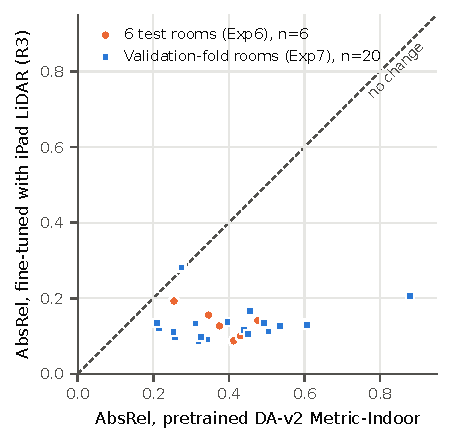
\includegraphics[width=\columnwidth]{finetune_absrel}
\caption{Per-room AbsRel against Faro depth: pretrained (x) vs.\ the LiDAR-teacher fine-tune R3 (y), for the six test
rooms (Exp.~6) and the \rsVN{} Validation-fold rooms (Exp.~7). Below the diagonal $=$ the fine-tune is better.}
\label{fig:finetuneabsrel}
\end{figure}

\begin{enumerate}
\item \textbf{The LiDAR-teacher fine-tune beats the pretrained model in every test room.} Chamfer
\SI{\rsMETRICCM}{cm}$\rightarrow$\SI{\rsFTLIDARALLCM}{cm} ($\rsMAINGAIN\times$; \SI{\rsMAINDIFFCM \pm \rsMAINDIFFSD}{cm}
better per room, \rsMAINWINS/\rsMAINN{} rooms, exact Wilcoxon $p=\rsMAINP$, the smallest attainable at $n=6$) and
\fscore{} \rsMETRICF$\rightarrow$\rsFTLIDARALLF{} (Tables~\ref{tab:main}, \ref{tab:mainscene}). The room where the
pretrained model fails worst (kitchen 45261556) is still R3's worst, but three times better.
\item \textbf{The 3D error falls because misplaced surfaces fall.} Accuracy (pred$\rightarrow$ref) drops
\SI{\rsMETRICACC}{cm}$\rightarrow$\SI{\rsFTLIDARALLACC}{cm}, more than completeness
(\SI{\rsMETRICCOMP}{cm}$\rightarrow$\SI{\rsFTLIDARALLCOMP}{cm}): the pretrained model builds the room but too far away
(it over-estimates distance by 15--31\,\%, \S\ref{sec:metric}); R3 brings the surfaces back near where they belong.
\item \textbf{The same holds in 2D on rooms that took part in nothing.} On the \rsVN{} Validation-fold rooms AbsRel
drops \rsVMETRICABSREL$\rightarrow$\rsVFTALLABSREL{} ($\rsVGAIN\times$; R3 better in \rsVWINS/\rsVN{} rooms, exact
Wilcoxon $p=\rsVP$) and $\delta_1$ rises \rsVMETRICDELTAONE$\rightarrow$\rsVFTALLDELTAONE{} (better in
\rsVWINSDELTA/\rsVN) (Table~\ref{tab:exp7}, Fig.~\ref{fig:finetuneabsrel}). The one room that does not improve is \rsVEXCEPT{}
(AbsRel \rsVEXCEPTPRE$\rightarrow$\rsVEXCEPTFT, $\delta_1$ \rsVEXCEPTDPRE$\rightarrow$\rsVEXCEPTDFT)---one of the
pretrained model's best rooms and R3's worst; in the other 19, R3's AbsRel is 21--64\,\% of the pretrained one
(median ratio over all \rsVN{} rooms \rsVMEDRATIO). The improvement is not a property of the six test rooms chosen at the start of the
project.
\item \textbf{It does not reach a sensor.} R3 is still $\sim$\SI{13}{cm} behind the iPad's LiDAR in Chamfer and
\SI{\rsFTALLGAPSPARSE}{cm} behind a per-frame fit on 200 sparse points; in 2D on the Validation fold LiDAR has AbsRel
\rsVLIDARABSREL{} vs.\ R3's \rsVFTALLABSREL. Fine-tuning fixes the scale of the \emph{domain}; it does not fix the
scale of \emph{the frame being looked at} (\S\ref{sec:whyft}). For a device with neither LiDAR nor trustworthy VIO
points, R3 is the only row in this paper that works without calibration at run time.
\end{enumerate}

\begin{figure*}[t]
\centering
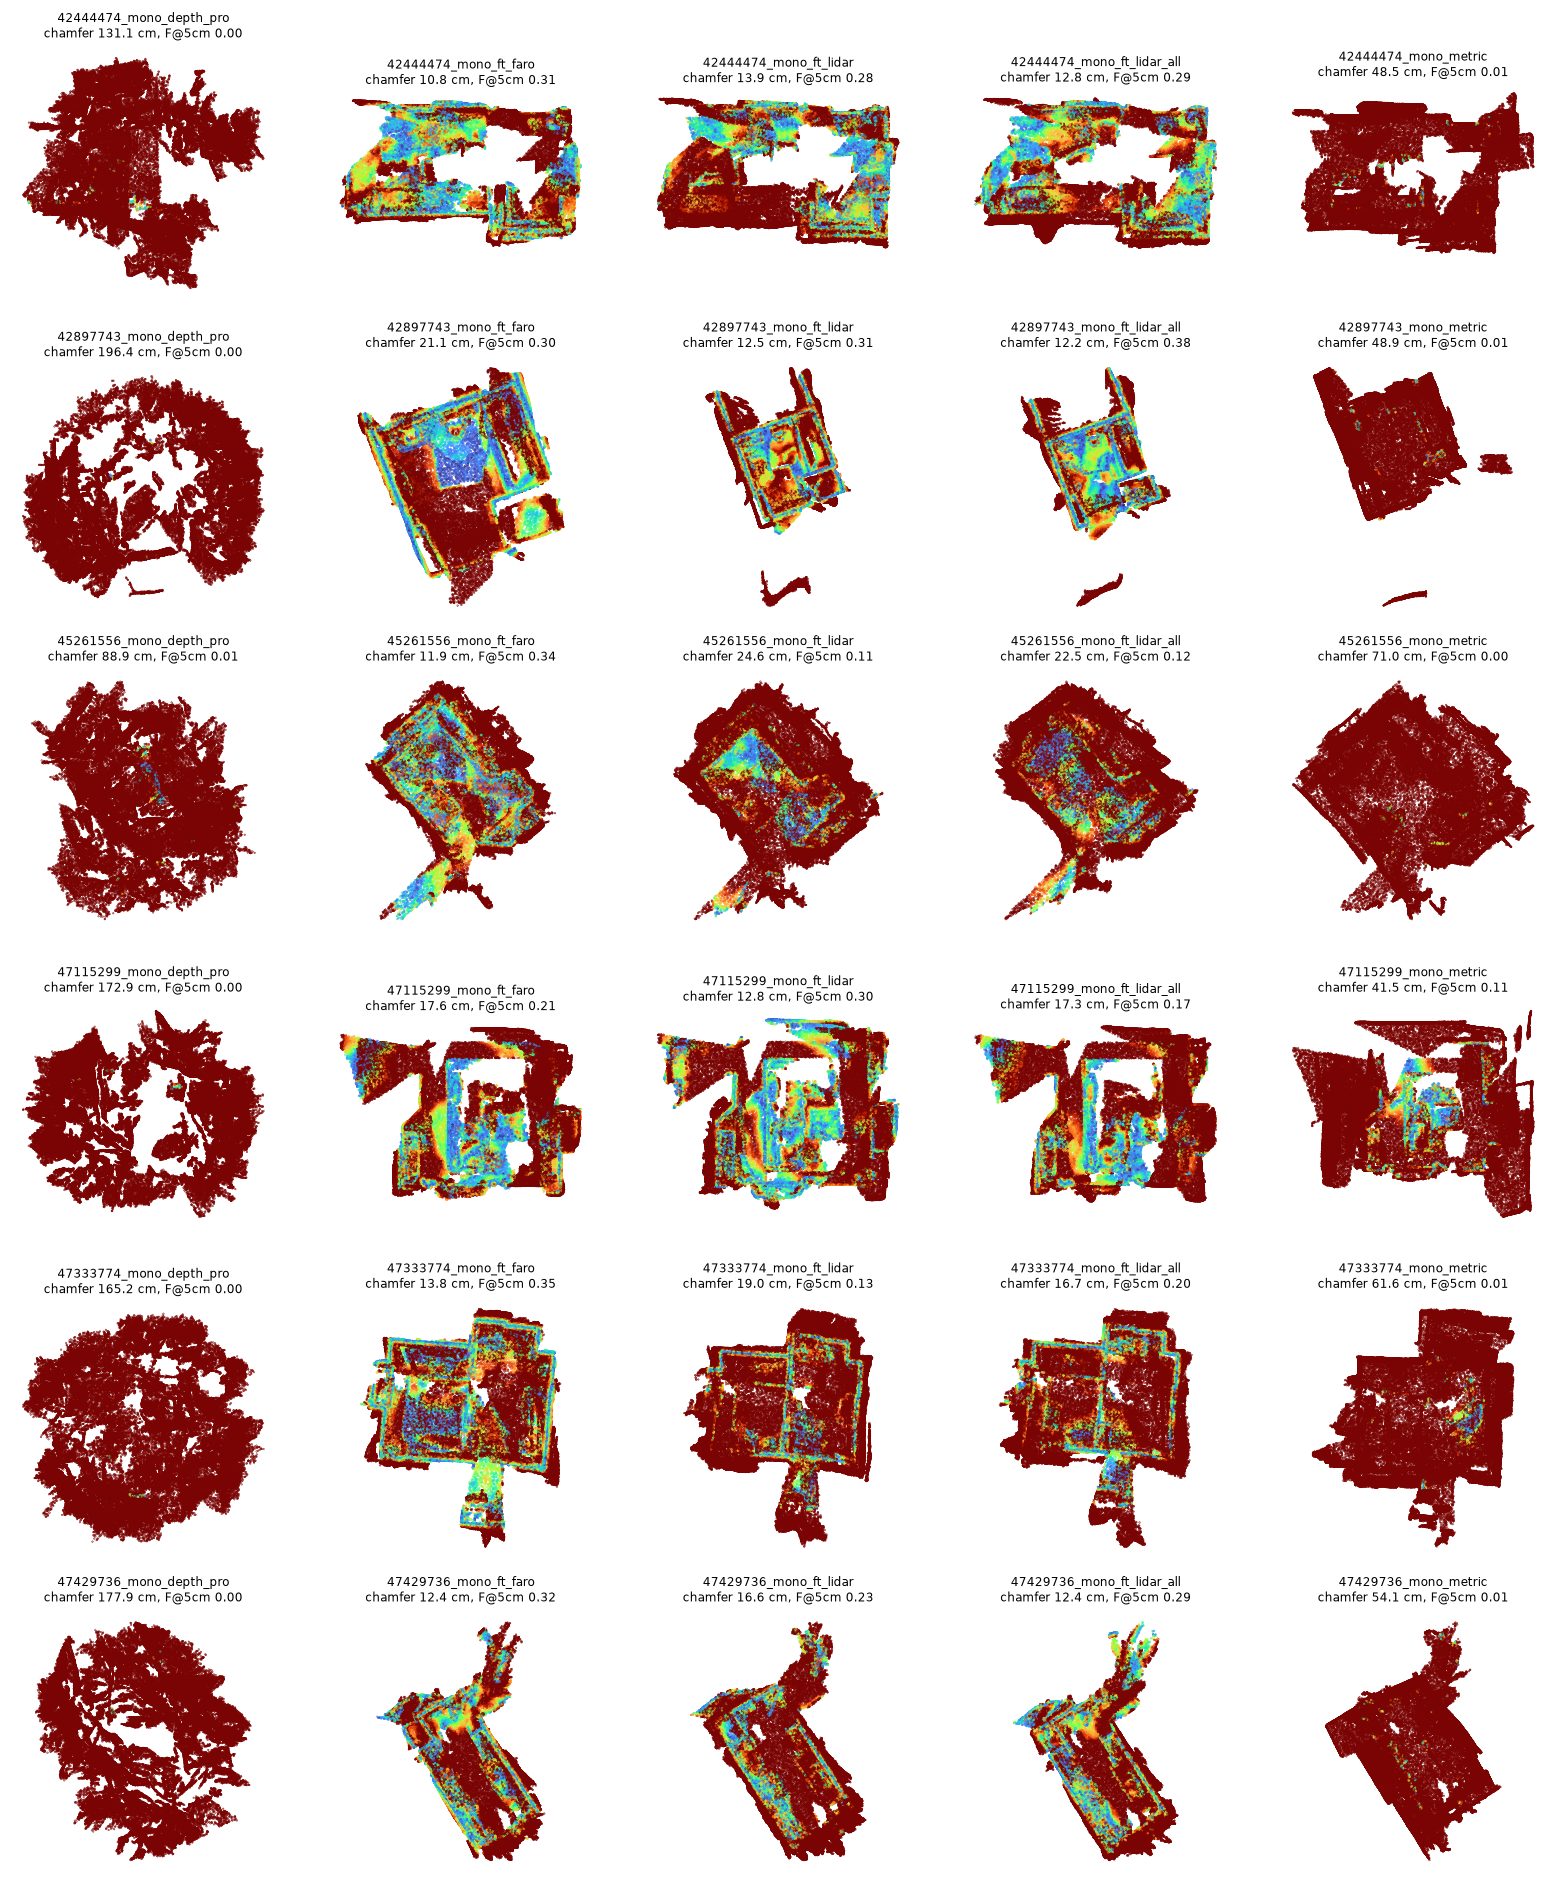
\includegraphics[width=\textwidth]{exp6_finetune_topdown_grid}
\caption{Exp.~6 top-down error maps (rows $=$ scenes, columns $=$ the three fine-tunes and the pretrained metric
model, colour $=$ distance to the reference, 0--\SI{10}{cm}). The pretrained column is red almost everywhere---the
room is built, at the wrong distance. After fine-tuning the walls and floor come back (blue/cyan) and the error
concentrates at object edges and far walls; where a fine-tune is weaker (45261556 and 47333774 with the LiDAR
teacher) it shows as a thick red rim around the room rather than a displaced room.}
\label{fig:exp6}
\end{figure*}

\subsection{Teacher ablation and a Level-0 baseline}\label{sec:finetune}
R3 is one of three fine-tunes with the same recipe (frozen DINOv2 backbone, DPT neck $+$ head, SiLog loss) that differ
in label and number of rooms: Faro \code{highres\_depth} on 10 rooms (R1, 3{,}594 frames), the iPad's LiDAR on the
same 10 rooms (R2, 8{,}656 frames), and LiDAR on 24 rooms (R3, the 10 $+$ 14 rooms with no laser scan at all,
19{,}896 frames). R1 and R2 share rooms but \emph{not frames}: Faro exists only on the frames Apple kept
($\sim$4~fps) whereas LiDAR accompanies every colour frame (every third taken, $\sim$10~fps), so at the same 6{,}000 steps
R2 sees $\sim$2.4$\times$ more distinct views than R1. The R1--R2 comparison therefore changes both the label and view
diversity. As a Level-0 reference the table also carries Depth Pro~\cite{depthpro}, a metric model of the other family
(\S\ref{sec:related}): no fine-tuning, and \emph{handed the camera's true focal length} (\SI{533}{px}) rather than the
one it predicts, which is the strongest form of that baseline.

\begin{table}[h]
\centering\small
\caption{Exp.~6, all rows: same pipeline, same six scenes, RGB-only, no alignment. Teacher $=$ the depth used as the training
label; none of these rows uses a depth sensor at test time.}
\label{tab:exp6}
\begin{adjustbox}{max width=\columnwidth}
\begin{tabular}{@{}llrrrr@{}}
\toprule
Model & Teacher & Chamfer & \textbf{F@5} & AbsRel & $\delta_1$ \\
\midrule
Depth Pro (intrinsics given) & --- & $\rsDEPTHPROCM \pm \rsDEPTHPROSD$ & \rsDEPTHPROF & \rsDEPTHPROABSREL & \rsDEPTHPRODELTAONE \\
Metric-Indoor (pretrained) & --- & $\rsMETRICCM \pm \rsMETRICSD$ & \rsMETRICF & \rsMETRICSIXABSREL & \rsMETRICSIXDELTAONE \\
$+$ fine-tune (R1) & Faro & $\mathbf{\rsFTFAROCM \pm \rsFTFAROSD}$ & \textbf{\rsFTFAROF} & \rsFTFAROABSREL & \rsFTFARODELTAONE \\
$+$ fine-tune (R2) & ARKit LiDAR & $\rsFTLIDARCM \pm \rsFTLIDARSD$ & \rsFTLIDARF & \rsFTLIDARABSREL & \textbf{\rsFTLIDARDELTAONE} \\
$+$ fine-tune (R3) & LiDAR, 24 scenes & $\rsFTLIDARALLCM \pm \rsFTLIDARALLSD$ & \rsFTLIDARALLF & \textbf{\rsFTLIDARALLABSREL} & \rsFTLIDARALLDELTAONE \\
\bottomrule
\end{tabular}
\end{adjustbox}
\end{table}

\begin{table}[h]
\centering\small
\caption{Exp.~6 Chamfer (cm) per scene; column order as in Table~\ref{tab:exp1scene}.}
\label{tab:exp6scene}
\begin{adjustbox}{max width=\columnwidth}
\begin{tabular}{@{}lrrrrrrr@{}}
\toprule
Teacher & 4244 & 4733 & 4711 & 4289 & 4742 & 4526 & mean \\
\midrule
Depth Pro (no fine-tune) & \rsDEPTHPROa & \rsDEPTHPROb & \rsDEPTHPROc & \rsDEPTHPROd & \rsDEPTHPROe & \rsDEPTHPROf & \rsDEPTHPROCM \\
none (pretrained) & \rsMETRICa & \rsMETRICb & \rsMETRICc & \rsMETRICd & \rsMETRICe & \rsMETRICf & \rsMETRICCM \\
Faro (R1) & \rsFTFAROa & \rsFTFAROb & \rsFTFAROc & \rsFTFAROd & \rsFTFAROe & \rsFTFAROf & \rsFTFAROCM \\
LiDAR (R2) & \rsFTLIDARa & \rsFTLIDARb & \rsFTLIDARc & \rsFTLIDARd & \rsFTLIDARe & \rsFTLIDARf & \rsFTLIDARCM \\
LiDAR $\times$24 (R3) & \rsFTLIDARALLa & \rsFTLIDARALLb & \rsFTLIDARALLc & \rsFTLIDARALLd & \rsFTLIDARALLe & \rsFTLIDARALLf & \rsFTLIDARALLCM \\
\bottomrule
\end{tabular}
\end{adjustbox}
\end{table}

\begin{enumerate}
\item \textbf{The laser teacher is not measurably better than the LiDAR teacher.} R1 \SI{\rsFTFAROCM}{cm}, R3
\SI{\rsFTLIDARALLCM}{cm} and R2 \SI{\rsFTLIDARCM}{cm} all lie within the across-room std (4.0--\SI{4.7}{cm}), and no
row wins every room (R1 beats R3 in three rooms, R3 wins two, one tie; Table~\ref{tab:exp6scene}). Given the frame
difference above, the honest claim is that a phone's depth sensor can replace the laser scanner as the teacher at no
measurable cost on these six rooms---not that the two are equal, or that either is better.
\item \textbf{Fourteen extra laser-free rooms do not help measurably} (R3 \SI{\rsFTLIDARALLCM}{cm} vs.\ R2
\SI{\rsFTLIDARCM}{cm}). R3 was the best run on the validation fold (AbsRel 0.133 vs.\ 0.142, measured during training under protocol~1) and is not the best here:
three validation rooms are too few to rank checkpoints this close (\S\ref{sec:limitations}). We take R3 as the main
model for reasons that do not depend on the test numbers: it is the only recipe that scales without a laser scanner,
and it was the best run on validation.
\item \textbf{Knowing the camera does not rescue metric depth.} Depth Pro, given the true intrinsics, is
\SI{\rsDEPTHPROCM}{cm} with \fscore{} \rsDEPTHPROF---worse than the pretrained DA-v2 Metric row it was meant to
improve on, and $\sim$10$\times$ the fine-tuned rows. Its structure is right (the surfaces of a frame land in the
right places relative to each other) and its distances are not: it predicts a \SI{48}{\degree} field of view where
the camera has \SI{62}{\degree}, and even after removing all scale per frame its AbsRel is 0.24--0.54 against
0.04--0.13 for DA-v2 Metric on the same frames. The failure is specific to this input---VGA
($640\times480$), close indoor range, motion blur---and we verified the wrapper against a synthetic room with exact
ground truth (\fscore{}-level agreement, AbsRel 0.008 after one scale), so it is the model on this data, not the
plumbing. The practical reading for a product team: a model that takes intrinsics is not a substitute for depth
labels from the target device.
\end{enumerate}

\subsection{Context, Exp.~1: the price of each depth source}\label{sec:exp1}
\begin{table*}[t]
\centering\small
\caption{Same pipeline, \SI{4}{cm} voxels, every Faro frame; only \code{depth.source} / \code{depth.aligner} change.
\code{sparse} $=$ per-frame fit on 200 LiDAR-sampled points (VIO proxy; upper bound of real VIO).}
\label{tab:exp1}
\begin{adjustbox}{max width=\textwidth}
\begin{tabular}{@{}llrrrrrrrr@{}}
\toprule
Depth source & Aligner & Chamfer & Acc. & Compl. & F@2 & \textbf{F@5} & F@10 & AbsRel (2D) & Time/scan (s) \\
\midrule
Faro laser (\code{gt}) & identity & $\mathbf{\rsGTCM \pm \rsGTSD}$ & \rsGTACC & \rsGTCOMP & \rsGTFtwo & \textbf{\rsGTF} & \rsGTFten & 0 & 1.6 \\
ARKit LiDAR (\code{lidar}) & identity & $\mathbf{\rsLIDARCM \pm \rsLIDARSD}$ & \rsLIDARACC & \rsLIDARCOMP & \rsLIDARFtwo & \textbf{\rsLIDARF} & \rsLIDARFten & \rsLIDARABSREL & 1.7 \\
DA-v2 L (\code{mono}) & \code{oracle\_frame} & $\mathbf{\rsORACLECM \pm \rsORACLESD}$ & \rsORACLEACC & \rsORACLECOMP & \rsORACLEFtwo & \textbf{\rsORACLEF} & \rsORACLEFten & \rsORACLEABSREL & 366 \\
DA-v2 L (\code{mono}) & \code{sparse\_points} & $\mathbf{\rsSPARSECM \pm \rsSPARSESD}$ & \rsSPARSEACC & \rsSPARSECOMP & \rsSPARSEFtwo & \textbf{\rsSPARSEF} & \rsSPARSEFten & \rsSPARSEABSREL & 360 \\
DA-v2 L (\code{mono}) & \code{per\_scene} & $\mathbf{\rsSCENECM \pm \rsSCENESD}$ & \rsSCENEACC & \rsSCENECOMP & \rsSCENEFtwo & \textbf{\rsSCENEF} & \rsSCENEFten & \rsSCENEABSREL & 351 \\
DA-v2 Metric-Indoor & identity & $\mathbf{\rsMETRICCM \pm \rsMETRICSD}$ & \rsMETRICACC & \rsMETRICCOMP & \rsMETRICFtwo & \textbf{\rsMETRICF} & \rsMETRICFten & \rsMETRICABSREL & 352 \\
\bottomrule
\end{tabular}
\end{adjustbox}
\end{table*}

\begin{table*}[t]
\centering\small
\caption{Chamfer (cm) per scene; column order as in Table~\ref{tab:scenes}. 42444474 is the development scene.}
\label{tab:exp1scene}
\begin{adjustbox}{max width=\textwidth}
\begin{tabular}{@{}lrrrrrrr@{}}
\toprule
Run & 42444474 kitchen/glass & 47333774 bedroom & 47115299 living & 42897743 bathroom & 47429736 bedroom$+$closets & 45261556 kitchen & mean \\
\midrule
gt & \rsGTa & \rsGTb & \rsGTc & \rsGTd & \rsGTe & \rsGTf & \rsGTCM \\
lidar & \rsLIDARa & \rsLIDARb & \rsLIDARc & \rsLIDARd & \rsLIDARe & \rsLIDARf & \rsLIDARCM \\
mono $+$ oracle & \rsORACLEa & \rsORACLEb & \rsORACLEc & \rsORACLEd & \rsORACLEe & \rsORACLEf & \rsORACLECM \\
mono $+$ sparse & \rsSPARSEa & \rsSPARSEb & \rsSPARSEc & \rsSPARSEd & \rsSPARSEe & \rsSPARSEf & \rsSPARSECM \\
mono $+$ per\_scene & \rsSCENEa & \rsSCENEb & \rsSCENEc & \rsSCENEd & \rsSCENEe & \rsSCENEf & \rsSCENECM \\
mono metric & \rsMETRICa & \rsMETRICb & \rsMETRICc & \rsMETRICd & \rsMETRICe & \rsMETRICf & \rsMETRICCM \\
\bottomrule
\end{tabular}
\end{adjustbox}
\end{table*}

What the table says directly:
\begin{enumerate}
\item \textbf{The pipeline loses $\sim$\SI{2}{cm}; LiDAR adds $\sim$\SI{1}{cm}.} The gap \code{lidar}$-$\code{gt} is
\SI{0.98 \pm 0.25}{cm} (0.66--1.33), the same in every room including the bathroom; \fscore{} 0.93 vs 0.97. The rows
differ clearly only at $\tau=$\SI{2}{cm} (0.54 vs 0.86): iPad LiDAR is wrong at the 2--\SI{4}{cm} level, not \SI{5}{cm}.
\item \textbf{Monocular depth with the right scale on every frame (oracle) is
\SI{\rsORACLEGAPLIDARCM \pm \rsORACLEGAPLIDARSD}{cm} behind LiDAR} (0.9--3.8). Bedroom 47333774 (3.8) and the bathroom
(3.4) are farthest; the development kitchen 42444474 (0.9) and kitchen 45261556 (1.6) closest---more room-dependent
than LiDAR's std suggests (\S\ref{sec:rooms}).
\item \textbf{Two hundred sparse metric points per frame recover the oracle.} \code{sparse\_points} lands at
\SI{\rsSPARSECM}{cm}, \SI{\rsSPARSEGAP}{cm} from the oracle and $\rsSPARSEVSSCENE\times$ better than one-off calibration,
with the same per-scene ordering as the oracle (Table~\ref{tab:exp1scene}). The remaining gap to LiDAR
(\SI{\rsSPARSEGAPLIDAR}{cm}) is shape, not scale.
\item \textbf{One calibration per scene (\code{per\_scene}) is $4.5 \pm 1.1\times$ worse than the oracle} (3.1--6.4$\times$),
and---importantly---\textbf{the absolute values cluster at 20--\SI{26}{cm} in every room} (std \SI{\rsSCENESD}{cm}, lower than
the oracle's): not one room failing, but a property of affine-invariant models with one scale per scene (\S\ref{sec:drift}).
\item \textbf{The metric model is worst (\SI{\rsMETRICCM}{cm}, $F$ \rsMETRICF) and most variable}
(42--\SI{71}{cm}); accuracy \SI{\rsMETRICACC}{cm} vs completeness \SI{\rsMETRICCOMP}{cm}: the surfaces are all there but
in the wrong place (\S\ref{sec:metric}). Kitchen 45261556, where mono$+$oracle is second best (\rsORACLEf), is where the
metric model is worst (\rsMETRICf)---right shape, wrong scale. This is the baseline of \S\ref{sec:main}: fine-tuning this
same model on ARKitScenes with a LiDAR teacher removes most of that error.
\end{enumerate}

\begin{figure*}[t]
\centering
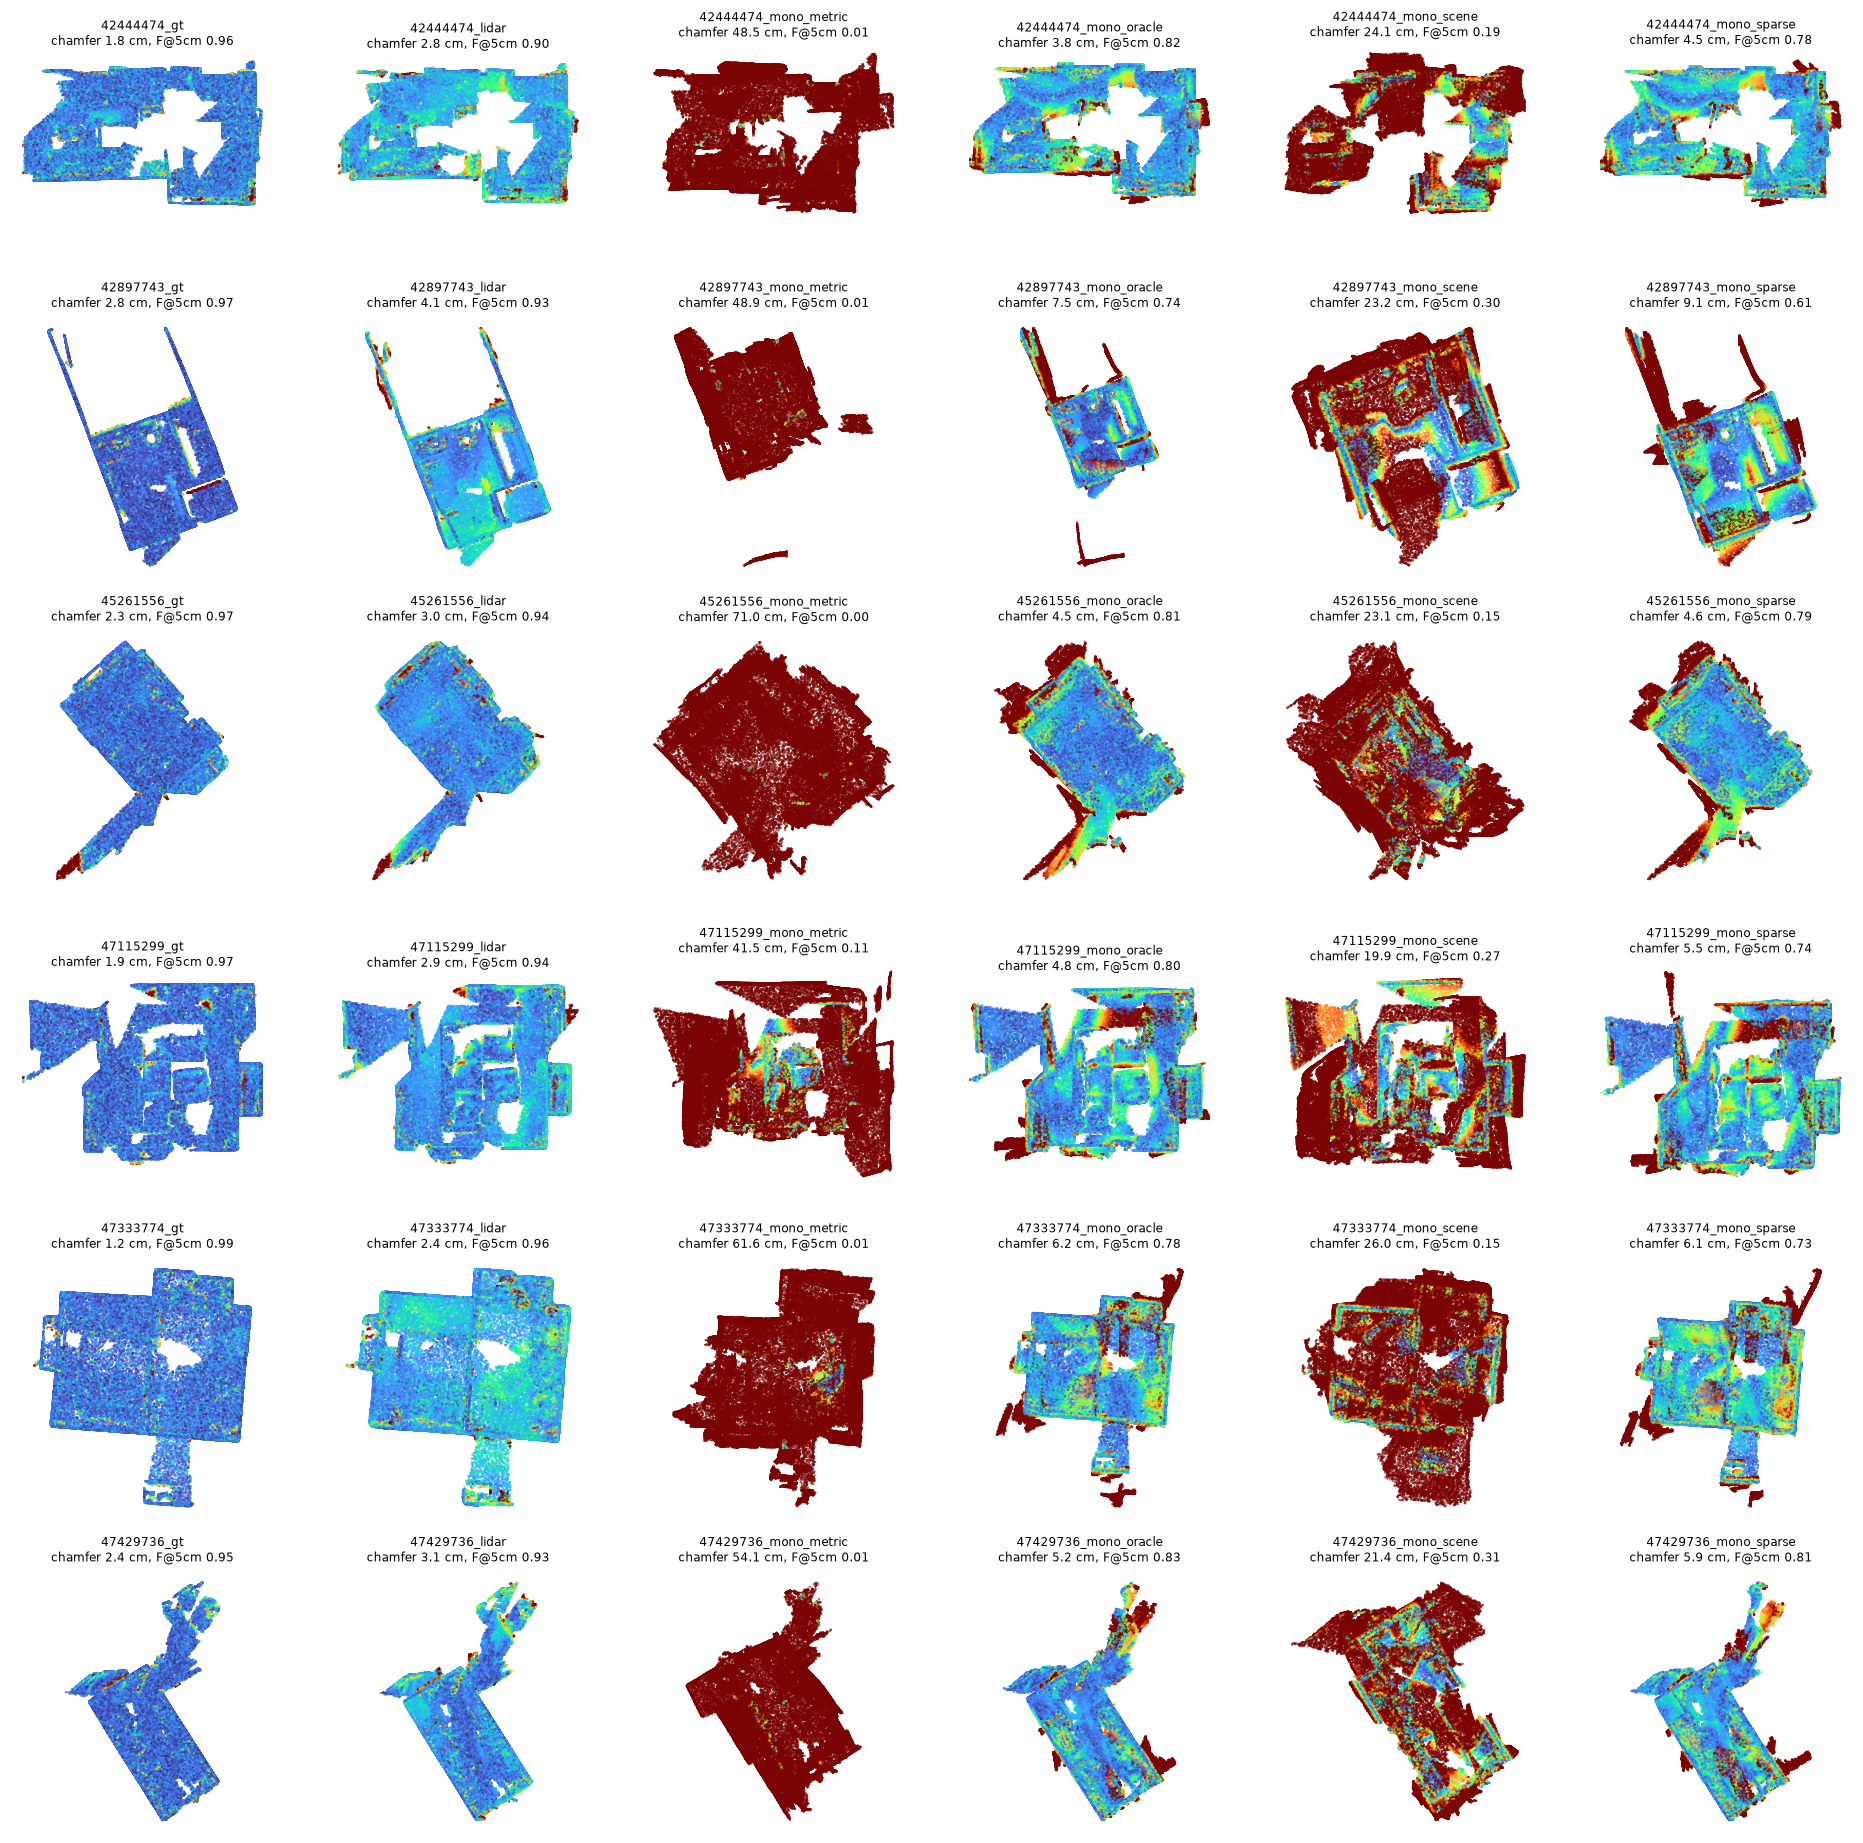
\includegraphics[width=\textwidth]{exp1_depth_source_topdown_grid}
\caption{Exp.~1 top-down error maps (rows $=$ scenes, columns $=$ runs, colour $=$ distance to reference,
0--\SI{10}{cm}). The gt/lidar columns are almost entirely blue ($<$\SI{2}{cm}); oracle and sparse show the same
yellow--red pattern at object edges and far walls; per\_scene has a red blob in the middle of every room (phantom surfaces from wrongly scaled
frames); metric is red almost everywhere.}
\label{fig:exp1}
\end{figure*}

\subsection{Context, Exp.~2: voxel size (GT depth)}
\begin{table}[h]
\centering\small
\caption{\code{depth.source: gt}, \code{sdf\_trunc} $=3\times$ voxel.}
\begin{adjustbox}{max width=\columnwidth}
\begin{tabular}{@{}lrrrrrrr@{}}
\toprule
Voxel & Chamfer & Acc. & Compl. & F@2 & F@5 & F@10 & Fusion (s) \\
\midrule
\SI{2}{cm} & $1.18 \pm 0.19$ & 1.05 & 1.31 & 0.92 & 0.99 & 1.00 & 2.5 \\
\textbf{\SI{4}{cm}} & $2.06 \pm 0.54$ & 1.29 & 2.83 & 0.86 & 0.97 & 0.99 & 1.5 \\
\SI{8}{cm} & $2.76 \pm 0.85$ & 1.74 & 3.79 & 0.76 & 0.93 & 0.97 & 1.3 \\
\bottomrule
\end{tabular}
\end{adjustbox}
\end{table}
Going from 2 to \SI{4}{cm} costs \SI{0.9}{cm} Chamfer, mostly completeness (1.3$\rightarrow$2.8: coarser corners and
edges), not accuracy (1.05$\rightarrow$1.29). From 4 to \SI{8}{cm} costs another \SI{0.7}{cm} and \fscore{} drops
0.97$\rightarrow$0.93---at \SI{8}{cm} discretisation exceeds LiDAR's own error. Fusion takes 1--\SI{3}{s} per scan at
every size (CPU, Open3D), so voxel size does not drive cost; inference does (\S\ref{sec:business}). \textbf{\SI{4}{cm}
is used throughout}: its discretisation (\SI{2.1}{cm}) is smaller than the depth-source effects being measured (LiDAR
$+1$, mono $+4$, per\_scene $+20$) and the mesh stays small enough for a phone.

\subsection{Context, Exp.~3: frame stride---how many frames per second to capture}\label{sec:stride}
Faro provides frames at $\sim$4.1~fps (2{,}352 frames / \SI{577}{s}); strides 1/5/10/20 therefore correspond to
$\approx$ 4 / 0.8 / 0.4 / 0.2~fps (391 / 78 / 40 / 20 frames per scan on average). Three rows per stride separate the
causes: GT control (coverage only), mono$+$oracle ($+$ model shape), mono$+$per\_scene ($+$ scale).
\begin{table*}[t]
\centering\small
\caption{Chamfer / accuracy / completeness (cm) and \fscore{} vs.\ stride.}
\begin{adjustbox}{max width=\textwidth}
\begin{tabular}{@{}lrrrrrrrr@{}}
\toprule
Stride ($\approx$fps) & Frames & GT: Ch / acc / comp & $F$ & mono oracle: Ch / acc / comp & $F$ & mono per\_scene: Ch / acc / comp & $F$ & mono time (s) \\
\midrule
1 (4) & \rsSTRGTONEN & \rsSTRGTONECM / \textbf{\rsSTRGTONEACC} / \rsSTRGTONECOMP & \rsSTRGTONEF & \rsSTRORACLEONECM / \rsSTRORACLEONEACC / \rsSTRORACLEONECOMP & \rsSTRORACLEONEF & \rsSTRSCENEONECM / \rsSTRSCENEONEACC / \rsSTRSCENEONECOMP & \rsSTRSCENEONEF & \rsSTRSCENEONESCAN \\
5 (0.8) & \rsSTRGTFIVEN & \rsSTRGTFIVECM / \textbf{\rsSTRGTFIVEACC} / \rsSTRGTFIVECOMP & \rsSTRGTFIVEF & \rsSTRORACLEFIVECM / \rsSTRORACLEFIVEACC / \rsSTRORACLEFIVECOMP & \rsSTRORACLEFIVEF & \rsSTRSCENEFIVECM / \rsSTRSCENEFIVEACC / \rsSTRSCENEFIVECOMP & \rsSTRSCENEFIVEF & \rsSTRSCENEFIVESCAN \\
10 (0.4) & \rsSTRGTTENN & \rsSTRGTTENCM / \textbf{\rsSTRGTTENACC} / \rsSTRGTTENCOMP & \rsSTRGTTENF & \rsSTRORACLETENCM / \rsSTRORACLETENACC / \rsSTRORACLETENCOMP & \rsSTRORACLETENF & \rsSTRSCENETENCM / \rsSTRSCENETENACC / \rsSTRSCENETENCOMP & \rsSTRSCENETENF & \rsSTRSCENETENSCAN \\
20 (0.2) & \rsSTRGTTWENTYN & \rsSTRGTTWENTYCM / \textbf{\rsSTRGTTWENTYACC} / \rsSTRGTTWENTYCOMP & \rsSTRGTTWENTYF & \rsSTRORACLETWENTYCM / \rsSTRORACLETWENTYACC / \rsSTRORACLETWENTYCOMP & \rsSTRORACLETWENTYF & \rsSTRSCENETWENTYCM / \rsSTRSCENETWENTYACC / \rsSTRSCENETWENTYCOMP & \rsSTRSCENETWENTYF & \rsSTRSCENETWENTYSCAN \\
\bottomrule
\end{tabular}
\end{adjustbox}
\end{table*}
\begin{itemize}
\item \textbf{Control:} GT accuracy is constant at 1.2--\SI{1.3}{cm} at every stride; the growing Chamfer
(\rsSTRGTONECM$\rightarrow$\SI{\rsSTRGTTWENTYCM}{cm}) is pure completeness. On this dataset stride measures \textbf{coverage}: a room swept once
develops holes below 1~fps.
\item \textbf{mono$+$oracle tracks the control plus a constant \SIrange{2.7}{3.3}{cm}}, and its accuracy
\emph{improves} with stride (\rsSTRORACLEONEACC$\rightarrow$\rsSTRORACLETWENTYACC): fewer frames means fewer
overlapping surfaces from different views; 2D AbsRel is \rsSTRORACLEONEABSREL{} at every stride, confirming the model
did not change.
\item \textbf{mono$+$per\_scene is flat at $\sim$\SI{23}{cm} up to stride 10}: at stride 5 it saves $5\times$ the time
(\rsSTRSCENEONESCAN$\rightarrow$\SI{\rsSTRSCENEFIVESCAN}{s}) at the same Chamfer (\rsSTRSCENEONECM{} vs.\
\rsSTRSCENEFIVECM), because the error is already dominated by scale. At stride 20
\code{per\_scene} fits on 10 of 20 frames (nearly a half-scene oracle), so that cell should not be over-interpreted.
\item \textbf{For the business:} with good depth (LiDAR) capture $\geq 1$~fps for a complete room (\fscore{} $>0.9$);
with mono$+$per\_scene, 0.8~fps gives the same result as 4~fps, $5\times$ faster---quality is capped by scale, not by
frame count.
\end{itemize}
At stride 20 every row has the same holes (areas the camera passed quickly): holes are a property of the scan, not of
the depth source.

\subsection{Context, Exp.~4: model size (oracle scale)}
\begin{table}[h]
\centering\small
\caption{\code{oracle\_frame} for every model, \SI{4}{cm}, every frame---pure ``shape,'' excluding the scale problem of \S5.1.}
\begin{adjustbox}{max width=\columnwidth}
\begin{tabular}{@{}lrrrrrrr@{}}
\toprule
Model & Params & Chamfer & F@5 & AbsRel & $\delta_1$ & ms/frame (MPS) & s/scan \\
\midrule
DA-v2 Large & 335M & $\mathbf{\rsDALARGECM \pm \rsDALARGESD}$ & \rsDALARGEF & \rsDALARGEABSREL & \rsDALARGEDELTAONE & 871 & \rsDALARGESCAN \\
DA-v2 Small & 25M & $\mathbf{\rsDASMALLCM \pm \rsDASMALLSD}$ & \rsDASMALLF & \rsDASMALLABSREL & \rsDASMALLDELTAONE & 121 & \rsDASMALLSCAN \\
MiDaS v2.1 small & 21M & $\mathbf{\rsMIDASCM \pm \rsMIDASSD}$ & \rsMIDASF & \rsMIDASABSREL & \rsMIDASDELTAONE & 27 & \rsMIDASSCAN \\
\bottomrule
\end{tabular}
\end{adjustbox}
\end{table}
L$\rightarrow$S: $13\times$ smaller, $6\times$ faster, $+$\SI{1.0}{cm} ($F$ \rsDALARGEF$\rightarrow$\rsDASMALLF);
every scene moves the same way except the bathroom, where Small is slightly \emph{better} (7.5$\rightarrow$7.1).
S$\rightarrow$MiDaS: similar parameter count, a further $3\times$ faster, but $2.1\times$ the Chamfer and $F$
\rsMIDASF---a matter of model generation (DA-v2 was trained with 62M unlabelled images), not size. At oracle scale
DA-v2 S (\SI{\rsDASMALLCM}{cm}) is still \SI{3.3}{cm} behind LiDAR (\rsLIDARCM).
Model size is not the main bottleneck: Table~\ref{tab:exp1} shows scale (oracle$\rightarrow$per\_scene,
$+$\SI{17.6}{cm}) costs $17\times$ more than model size (L$\rightarrow$S, $+$\SI{1.0}{cm}).

\subsection{Context, Exp.~5: does LiDAR confidence help?}\label{sec:exp5}
ARKit ships a $\{0,1,2\}$ confidence map with every LiDAR frame. Masking or weighting by it is the cheapest possible
improvement to the ``iPhone~Pro today'' row.
\begin{table}[h]
\centering\small
\caption{\code{lidar} row with confidence masking / integer TSDF weights (\SI{4}{cm}, every frame).}
\begin{adjustbox}{max width=\columnwidth}
\begin{tabular}{@{}lrrrr@{}}
\toprule
Variant & Chamfer & Acc. & Compl. & F@5 \\
\midrule
all pixels, weight 1 (Exp.~1) & $3.04 \pm 0.57$ & 2.23 & 3.85 & 0.93 \\
mask confidence $\geq 1$ & \rsCONFONECM & \rsCONFONEACC & \rsCONFONECOMP & \rsCONFONEF \\
mask confidence $= 2$ & \rsCONFTWOCM & \rsCONFTWOACC & \rsCONFTWOCOMP & \rsCONFTWOF \\
weights $[0,1,2]$ & \rsWZOTCM & \rsWZOTACC & \rsWZOTCOMP & \rsWZOTF \\
weights $[1,2,4]$ & \rsWOTFCM & \rsWOTFACC & \rsWOTFCOMP & \rsWOTFF \\
\bottomrule
\end{tabular}
\end{adjustbox}
\end{table}
Nothing moves: dropping confidence-0 pixels or weighting by tier changes Chamfer by $\leq$\SI{0.03}{cm}; keeping only
confidence-2 pixels improves accuracy slightly (2.23$\rightarrow$2.08) but loses completeness (3.85$\rightarrow$5.23,
worst in the closet-heavy bedroom 47429736: 3.1$\rightarrow$5.8). The \SI{1}{cm} LiDAR$-$laser gap is not a
low-confidence-pixel problem; it is the sensor's resolution and its 2--\SI{4}{cm} noise everywhere.

\subsection{Numbers carried into \S6--7}
\begin{table}[h]
\centering\small
\begin{tabularx}{\columnwidth}{@{}lX@{}}
\toprule
Question & Number \\
\midrule
\textbf{R3 vs.\ pretr.\ (3D, 6 rooms)} & \textbf{\SI{\rsMETRICCM}{cm} $\rightarrow$ \SI{\rsFTLIDARALLCM}{cm}, \fscore{} \rsMETRICF{} $\rightarrow$ \rsFTLIDARALLF, every room better} \\
\textbf{R3 vs.\ pretr.\ (2D, 6 rooms)} & \textbf{AbsRel \rsMETRICSIXABSREL{} $\rightarrow$ \rsFTLIDARALLABSREL, $\delta_1$ \rsMETRICSIXDELTAONE{} $\rightarrow$ \rsFTLIDARALLDELTAONE} \\
\textbf{R3 vs.\ pretr.\ (2D, \rsVN{} rooms)} & \textbf{AbsRel \rsVMETRICABSREL{} $\rightarrow$ \rsVFTALLABSREL, better in \rsVWINS/\rsVN} \\
Faro vs.\ LiDAR teacher & \SI{\rsFTFAROCM}{cm} / \SI{\rsFTLIDARCM}{cm} / \SI{\rsFTLIDARALLCM}{cm} (R1/R2/R3): not measurably different \\
pipeline loss at \SI{4}{cm} & \SI{2.1 \pm 0.5}{cm} \\
iPad LiDAR vs laser & $+$\SI{1.0 \pm 0.3}{cm}, \fscore{} 0.93 (confidence weighting: no change) \\
mono ceiling (scale known per frame) & $+$\SI{\rsORACLEGAPLIDARCM \pm \rsORACLEGAPLIDARSD}{cm} from LiDAR, \fscore{} \rsORACLEF \\
mono with 200 sparse points/frame & \SI{\rsSPARSECM}{cm}, \fscore{} \rsSPARSEF{} (\SI{\rsSPARSEGAP}{cm} from oracle) \\
price of ``one scale per scene'' & $4.5\times$ oracle $\rightarrow$ \SI{\rsSCENECM}{cm}, \fscore{} \rsSCENEF \\
intrinsics-conditioned model (Depth Pro) & \SI{\rsDEPTHPROCM}{cm}, \fscore{} \rsDEPTHPROF{} --- intrinsics do not replace in-domain labels \\
voxel 2$\rightarrow$4$\rightarrow$\SI{8}{cm} & 1.2 $\rightarrow$ 2.1 $\rightarrow$ \SI{2.8}{cm} \\
fps needed (LiDAR/GT) & $\geq 0.8$~fps for \fscore{} $\geq 0.9$; 0.4~fps leaves 0.83 \\
L$\rightarrow$S$\rightarrow$MiDaS & \rsDALARGECM $\rightarrow$ \rsDASMALLCM $\rightarrow$ \SI{\rsMIDASCM}{cm} at 871 $\rightarrow$ 121 $\rightarrow$ 27 ms/frame \\
\bottomrule
\end{tabularx}
\end{table}

\section{Discussion}\label{sec:discussion}
Material: per-frame scale analysis on 6 scenes (\code{analyze\_scale\_drift.py}, stride 5, 471 frames), the failure-frame
study of scene 42444474, and Tables~\ref{tab:main}--\ref{tab:exp1scene}. Per-frame AbsRel uses protocol~2.

\subsection{Why the LiDAR-teacher fine-tune works---and why it is not enough}\label{sec:whyft}
We ran the per-frame analysis of \S\ref{sec:metric} on R3 as well (every fifth frame of the six test rooms, 471
frames): per frame, the GT/pred ratio (median over the frame) and AbsRel under different amounts of scale help
(Table~\ref{tab:whyft}).
\begin{table*}[t]
\centering\small
\caption{Per-frame scale of the pretrained metric model vs.\ the LiDAR-teacher fine-tune R3, six test rooms, every fifth
frame. AbsRel uses protocol~2.}
\label{tab:whyft}
\begin{tabularx}{\textwidth}{@{}lllX@{}}
\toprule
 & Pretrained & \textbf{R3} & Meaning \\
\midrule
median(GT / pred) per room & 0.69--0.85 & \textbf{0.93--1.21} & \textbf{the domain bias is gone}: pretrained is 15--31\,\% too far in every room; R3 is within $\sim$20\,\% and not always in the same direction \\
per-frame swing within a room (p95/p5 of GT/pred) & 1.33--1.79$\times$ (mean 1.55) & 1.26--1.92$\times$ (mean 1.52) & \textbf{fine-tuning does not reduce the per-frame swing} \\
AbsRel, raw & 0.381 & \textbf{0.134} & \\
AbsRel with one $(S,T)$ per room fitted on 10 GT frames & 0.127 & 0.117 & pretrained $+$ per-room GT calibration $\approx$ R3 with no calibration at all \\
AbsRel with the right scale on every frame (one factor) & 0.045 & 0.051 & the per-frame scale is almost all of R3's remaining error \\
AbsRel, oracle $(s,t)$ per frame & 0.035 & 0.042 & shape hardly changes (frozen encoder) \\
\bottomrule
\end{tabularx}
\end{table*}
\begin{enumerate}
\item \textbf{Fine-tuning works because it learns the domain's multiplier.} R3 with no calibration (AbsRel 0.134) is on
par with the pretrained model given a per-room scale fitted on ground truth (0.127): what a one-off calibration per room
provides has been moved into the head's weights, using LiDAR labels from other rooms. With the encoder frozen, shape
barely changes (oracle 0.035 $\rightarrow$ 0.042); the whole gain is scale.
\item \textbf{It is not enough because the per-frame swing remains.} Within one room, frames at p5 and p95 still need
factors $\sim$1.5$\times$ apart, as before fine-tuning, and that swing is nearly all of what is left: with the right
scale on every frame R3's AbsRel drops from 0.134 to 0.051 (90\,\% of the way to the oracle), whereas one $(S,T)$ per
room only reaches 0.117. The failing frames are those of \S\ref{sec:drift}--\ref{sec:metric} (blank walls, white
cabinets, close downward views with no size cue). The missing information is not in a single image and does not come
from a better teacher (the laser teacher does no better, \S\ref{sec:finetune}); it has to come from metric data at run
time.
\item \textbf{Fine-tuning and per-frame metric points are complementary, not alternatives.} Fine-tuning removes the
domain bias with nothing at run time (\SI{\rsMETRICCM}{cm} $\rightarrow$ \SI{\rsFTLIDARALLCM}{cm}); per-frame sparse
points remove the per-frame swing (relative model: \SI{\rsSCENECM}{cm} $\rightarrow$ \SI{\rsSPARSECM}{cm},
\S\ref{sec:exp1}). The 2D bound for combining them is the 0.051 ``right scale on every frame'' row above; measuring
R3 $+$ \code{sparse\_points} in 3D is the most direct next step (\S\ref{sec:limitations}).
\end{enumerate}

\subsection{Why per\_scene loses to the oracle by $4.5\times$: the model's scale follows what is in the frame, not time}\label{sec:drift}
An affine-invariant model promises $\text{disparity} \approx a\cdot(1/\text{depth}) + b$ with $(a,b)$ depending on
the image. If $(a,b)$ were constant over a scan, one calibration (\code{per\_scene}) would equal the oracle. We measured
how constant it is by refitting $(s,t)$ on every fifth frame (Fig.~\ref{fig:drift}, Table~\ref{tab:drift}).
\begin{figure*}[t]
\centering
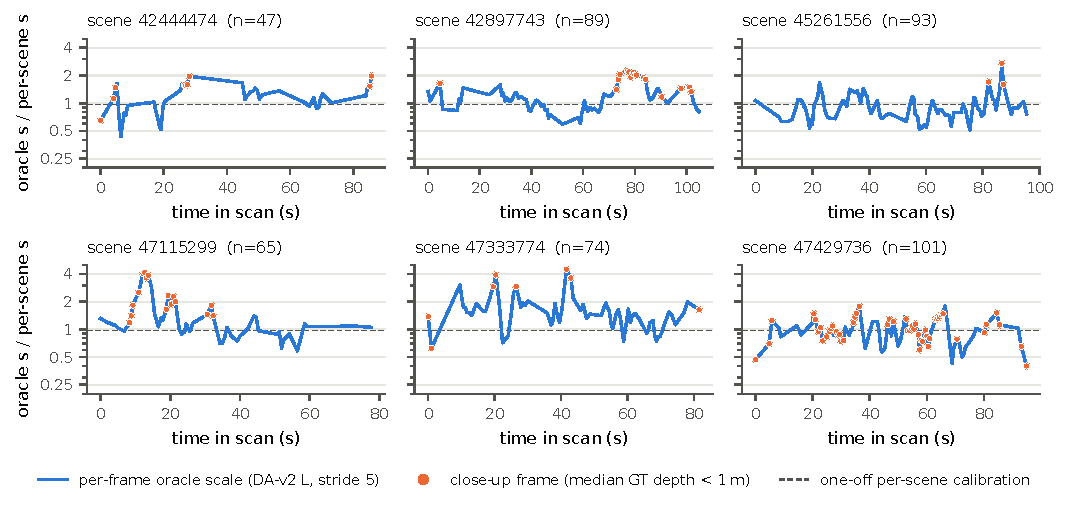
\includegraphics[width=\textwidth]{scale_drift_timeline}
\caption{Per-frame oracle scale divided by the per-scene scale, over time, for DA-v2 Large on all six scenes (log axis;
1.0 $=$ the one-off calibration was right for that frame). Orange dots mark close-up frames (median GT depth
$<$\SI{1}{m}). The ratio swings by $2$--$4\times$ within every scan with no monotone trend.}
\label{fig:drift}
\end{figure*}
\begin{table*}[t]
\centering\small
\caption{DA-v2 Large, per-scene values across the six scenes.}
\label{tab:drift}
\begin{tabularx}{\textwidth}{@{}lXX@{}}
\toprule
 & Range over scenes & Meaning \\
\midrule
$s$ p95 / p5 within one scene & \textbf{2.6--4.9$\times$} & the central 90\% of frames need scales 3--5$\times$ apart \\
$s$ p75 / p25 & 1.47--1.56 & even the middle half swings $\pm25\%$ \\
corr($s$, time) & $-0.33 \ldots +0.30$ (sign flips) & \textbf{not cumulative drift}: no direction \\
corr($s$, frame's median depth) & \textbf{$-0.27 \ldots -0.75$ (negative in every scene)} & close-up frames need a different $s$: view-dependent \\
AbsRel oracle $\rightarrow$ per\_scene & 0.032 $\rightarrow$ 0.239 (\textbf{7.5$\times$}) & in 2D, before fusion, one scale costs $7\times$ \\
per\_scene without close-ups ($<$\SI{1}{m}) & 0.152 (still $5\times$ oracle) & close-ups hurt but are not the only cause \\
scale-only per frame, depth space & 0.331 (worse than per\_scene) & a disparity shift is needed in every scene \\
\bottomrule
\end{tabularx}
\end{table*}
\begin{figure}[t]
\centering
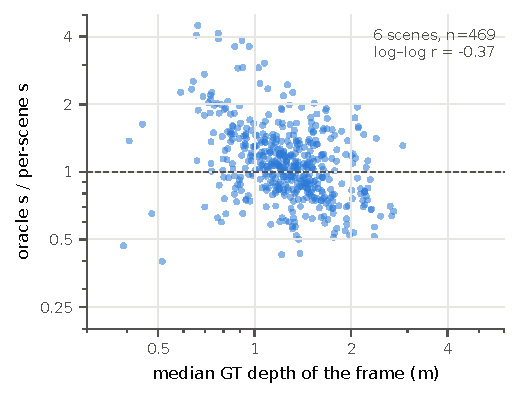
\includegraphics[width=\columnwidth]{scale_vs_depth}
\caption{The same ratio against the frame's median GT depth, all scenes pooled: the scale a frame needs correlates with
how close the camera is to what it sees.}
\label{fig:scalevsdepth}
\end{figure}
Three consequences:
\begin{enumerate}
\item \textbf{No number of fit frames helps \code{per\_scene}}: the $(S,T)$ fitted on 10 spread frames already lands
within $\pm13\%$ of the median oracle scale in five of the six scenes (0.87--1.17$\times$; the exception, 47333774,
is 0.67$\times$). The problem is that the median does not apply to most frames, not that it is estimated badly.
\item \textbf{A $7.5\times$ per-frame error becomes a $4.5\times$ 3D error} not because TSDF averages it out but because
the error concentrates in a minority of frames: frames with per\_scene AbsRel $>1$ (placed $\geq2\times$ wrong) are
downward shots of table-tops or floor at 0.5--\SI{0.8}{m} and frame-filling blank walls or cabinets. These frames carry
no size cue, so the model guesses disparity at ``room scale''; multiplied by the room's $(S,T)$, a table at \SI{0.5}{m}
lands at 1.5--\SI{2}{m} as a phantom surface in the middle of the room---the red blob in every per\_scene panel of
Fig.~\ref{fig:exp1}.
\item \textbf{The effect is general, not a property of the development scene}: 47429736 (bedroom$+$closets) has
close-ups in 53/101 frames yet per\_scene AbsRel 0.197, the same as a scene with 3/93 (45261556: 0.172); and the five
unseen scenes give per\_scene Chamfer 19.9--\SI{26.0}{cm}, bracketing 42444474 (24.1).
\end{enumerate}
\textbf{System implication.} The assumption ``one scale per scene'' is false for this model family on real room video.
Two ways remain: (a) \emph{per-frame} metric data---3D feature points from VIO, which ARKit/ARCore deliver with the pose
anyway (\code{sparse\_points}); or (b) drop or down-weight cue-less frames before fusion---cheaper, but removing
close-ups still leaves $4\times$ the oracle, so it can only supplement (a). Exp.~1 confirms (a): 200 points per frame
bring the row to \SI{\rsSPARSECM}{cm}, \SI{\rsSPARSEGAP}{cm} from the oracle, with the same per-scene ordering. The per-frame
fit needs no history and tolerates frames without points by carrying the previous $(s,t)$, exactly what a tracker
outage looks like.

\subsection{Why the ``metric'' model gives \SI{\rsMETRICCM}{cm}: right on average, wrong per frame}\label{sec:metric}
DA-v2 Metric-Indoor should output metres directly. Per-frame analysis over the six scenes:
\begin{table*}[t]
\centering\small
\begin{tabularx}{\textwidth}{@{}lXX@{}}
\toprule
 & Range over scenes & Meaning \\
\midrule
median(GT / pred) per scene & 0.69--0.85 & the model says 15--31\% too far on average (per-scene bias) \\
GT / pred within a scene & e.g.\ 0.41--0.86, 0.43--1.35 & frames in one room are wrong from $-59\%$ to $+35\%$ \\
oracle $t$ in inverse space & $-0.11 \ldots -0.02$ ($\approx 0$) & \textbf{no shift}: the shape is right in the affine sense \\
AbsRel raw $\rightarrow$ scale-only/frame $\rightarrow$ oracle $(s,t)$ & 0.381 $\rightarrow$ \textbf{0.045} $\rightarrow$ 0.035 & one scalar per frame recovers 97\% of the gap \\
AbsRel with one $(S,T)$ per scene & 0.127 & like per\_scene for the relative model: the median is not enough---and what fine-tuning moves into the weights (\S\ref{sec:whyft}) \\
\bottomrule
\end{tabularx}
\end{table*}
In 3D the same surface from several frames is placed at several distances and TSDF averages them into a thick slab:
accuracy \SI{\rsMETRICACC}{cm} but completeness \SI{\rsMETRICCOMP}{cm} (Table~\ref{tab:exp1})---everything is there,
in the wrong place. The worst scene (kitchen 45261556, \SI{\rsMETRICf}{cm}) is among the model's best shapes under the
oracle (\SI{\rsORACLEf}{cm}), confirming a pure scale effect. The worst frames in every scene look alike: a single flat, uniformly coloured surface
filling the frame (white cabinets, tiles) with nothing distant to compare against---the model's prior pushes flat
surfaces away. \textbf{Implication:} a metric model does not remove calibration; it reduces it from two parameters per
frame $(s,t)$ to \textbf{one} $(s)$, which is a real advantage: a handful of VIO points suffice to fit one scalar
stably, whereas $(s,t)$ needs points spread over the depth range. The other way to get that scalar is to put it in
the weights: fine-tuning the same checkpoint with LiDAR labels from real iPad frames (R3, \num{19896} frames) moves the
row to \SI{\rsFTLIDARALLCM}{cm} with no run-time fit at all (\S\ref{sec:main}), the deployable answer for a device that
has neither LiDAR nor reliable VIO points; \S\ref{sec:whyft} shows that what it fixes is the domain bias, while the
per-frame swing remains.

\subsection{Which rooms are hard, and for whom}\label{sec:rooms}
Ranking scenes by Chamfer per row (Table~\ref{tab:exp1scene}): Faro/LiDAR go from bedroom 47333774 (easiest) to the
bathroom (\rsGTb--\rsGTd{} / \rsLIDARb--\rsLIDARd); mono$+$oracle from the development kitchen 42444474 and kitchen
45261556 to the bathroom (\rsORACLEa--\rsORACLEd); mono$+$per\_scene from living room 47115299 to bedroom 47333774
(\rsSCENEc--\rsSCENEb).
\begin{itemize}
\item \textbf{The bathroom is hard for every source} (LiDAR $+1.3$ from Faro, oracle $+3.4$ from LiDAR): the mirror yields
phantom depth for LiDAR and model alike, glossy tiles reflect; it is the only scene where the oracle fit produced
$s \leq 0$ on some frames (a frame-filling mirror). If the target market is bathroom renovation, this paper's averages
are optimistic.
\item \textbf{Standard bedroom 47333774 is easiest for LiDAR but second-hardest for mono} (oracle \rsORACLEb): a small room
scanned close to walls and bed leaves most frames at 1--\SI{2}{m} of blank wall with no cue. Rooms with ``lots of
stuff'' (kitchen 45261556: 10 cabinets; living room: 4 tables, 2 sofas) are easy for mono---the model likes objects of
known size.
\item The mono difficulty order does not match LiDAR's $\Rightarrow$ \textbf{``hard scenes'' must be assessed per
source}; LiDAR experience does not predict where mono fails.
\end{itemize}

\subsection{Visible only in 3D: mono disagrees with itself across views}
Exp.~3 shows what 2D metrics cannot: reducing frames from 391 to 20 (stride 20) \textbf{improves mono$+$oracle accuracy
from \rsSTRORACLEONEACC{} to \SI{\rsSTRORACLETWENTYACC}{cm}} while 2D AbsRel stays at
\rsSTRORACLEONEABSREL--\rsSTRORACLETWENTYABSREL{} and GT accuracy at \rsSTRGTONEACC--\SI{\rsSTRGTTWENTYACC}{cm}. Even with every frame perfectly scaled,
the shape of the same surface from different views \textbf{disagrees} at the $\sim$\SI{2}{cm} level, and fusing more
frames thickens the surface rather than sharpening it---the multi-view consistency LiDAR has and a single-image model
lacks. This is the part of the oracle$\rightarrow$LiDAR gap (\SI{\rsORACLEGAPLIDARCM}{cm}) that scale alignment cannot fix, and the
reason systems like SimpleRecon use multi-image cost volumes (\S\ref{sec:related-mv}). The sparse row inherits it: its remaining gap to
LiDAR (\SI{\rsSPARSEGAPLIDAR}{cm}) is this shape term.

\subsection{Conclusions for system design}
\begin{table*}[t]
\centering\small
\begin{tabularx}{\textwidth}{@{}XX@{}}
\toprule
Assumed beforehand & What the data say \\
\midrule
mono's problem is coarse shape & shape is \SI{\rsORACLEGAPLIDARCM}{cm} behind LiDAR; scale is \SI{18}{cm} behind \\
one calibration per room suffices & no: \SI{\rsSCENECM}{cm} in every room; scale is view-dependent \\
a metric model removes the scale problem & no: but it reduces it to one parameter per frame \\
a metric model cannot be fixed without a laser scanner & largely can: a phone-LiDAR teacher takes it from \SI{\rsMETRICCM}{cm} to \SI{\rsFTLIDARALLCM}{cm} in every room (\S\ref{sec:main}); the rest is per-frame scale (\S\ref{sec:whyft}) \\
a few sparse metric points cannot fix a dense map & they can: 200 points/frame $\rightarrow$ within \SI{\rsSPARSEGAP}{cm} of the oracle \\
a bigger model means a more accurate room & $+$\SI{1.0}{cm} S$\rightarrow$L vs.\ $+$\SI{17.6}{cm} from scale \\
more frames mean more accuracy & more frames mean more coverage; mono accuracy improves with fewer frames \\
LiDAR confidence maps are free accuracy & no measurable gain from masking or weighting (Exp.~5) \\
LiDAR's hard scenes are mono's hard scenes & no (blank bedroom: hard for mono, easy for LiDAR) \\
\bottomrule
\end{tabularx}
\end{table*}

\section{Business Implications}\label{sec:business}
Numbers from \S\ref{sec:results}; times are Apple Silicon / MPS and serve only for ratios (\S\ref{sec:limitations}).

\subsection{The one number a decision-maker needs: ``how crooked is the room'' per use case}
Table~\ref{tab:usecase} translates Table~\ref{tab:exp1} into product language, requiring that a use case have
$\geq 90\%$ of the surface within $\tau$ of the truth (recall@$\tau$).
\begin{table*}[t]
\centering\small
\caption{Recall@$\tau$ averaged over 6 scenes. \checkmark\ $\geq 0.9$, $\sim$ 0.75--0.9, $\times$ $< 0.75$.}
\label{tab:usecase}
\begin{adjustbox}{max width=\textwidth}
\begin{tabular}{@{}llrrrrrrr@{}}
\toprule
Use case & $\tau$ & Faro & iPad LiDAR & mono $+$ oracle & mono $+$ sparse & mono $+$ per\_scene & mono ft (LiDAR) & mono metric \\
\midrule
room overview / virtual walk-through & \SI{10}{cm} & \checkmark\ \rsGTRten & \checkmark\ \rsLIDARRten & \checkmark\ \rsORACLERten & \checkmark\ \rsSPARSERten & $\times$ \rsSCENERten & $\times$ \rsFTLIDARRten & $\times$ \rsMETRICRten \\
furniture placement / space planning & \SI{5}{cm} & \checkmark\ \rsGTRfive & \checkmark\ \rsLIDARRfive & $\sim$ \rsORACLERfive & $\sim$ \rsSPARSERfive & $\times$ \rsSCENERfive & $\times$ \rsFTLIDARRfive & $\times$ \rsMETRICRfive \\
floor-area sale / renovation (walls, trim) & \SI{2}{cm} & $\sim$ \rsGTRtwo & $\times$ \rsLIDARRtwo & $\times$ \rsORACLERtwo & $\times$ \rsSPARSERtwo & $\times$ \rsSCENERtwo & $\times$ \rsFTLIDARRtwo & $\times$ \rsMETRICRtwo \\
\bottomrule
\end{tabular}
\end{adjustbox}
\end{table*}
\begin{itemize}
\item \textbf{iPad~Pro today is enough for ``furniture placement'' but not for ``renovation measurement'':} at
\SI{2}{cm} LiDAR reaches only half, and even Faro through this pipeline reaches 0.84 (the \SI{4}{cm} voxel eats it;
\S5.2 shows \SI{2}{cm} voxels reach 0.92). A product promising centimetre accuracy needs finer voxels plus multiple
LiDAR passes, or a laser. Confidence weighting does not move this (Exp.~5).
\item \textbf{Devices without LiDAR serve no use case} with one-off calibration (per\_scene \SI{\rsSCENECM}{cm}) or a
raw metric model (\SI{\rsMETRICCM}{cm}). Fine-tuning that metric model on data a phone can collect itself buys the
``rough overview'' tier without any run-time calibration (\SI{\rsFTLIDARCM}{cm}, \S\ref{sec:finetune}) but not the
``furniture placement'' tier.
\item \textbf{With per-frame sparse points the same device reaches \SI{\rsSPARSECM}{cm}, recall@\SI{5}{cm} \rsSPARSERfive}---the
``furniture placement'' tier at a level close to iPad~Pro, and the mono ceiling (oracle \SI{\rsORACLECM}{cm}) is only
\SI{\rsORACLEGAPLIDARCM}{cm} behind LiDAR. This is the gap to invest in, not the model.
\end{itemize}

\subsection{Where to invest: scale first, model second}
\begin{table*}[t]
\centering\small
\caption{What eats mono's error, six scenes.}
\begin{tabularx}{\textwidth}{@{}lXXX@{}}
\toprule
Error source & Size (Chamfer) & Remedy & Cost \\
\midrule
one scale per scene $\rightarrow$ per frame & \textbf{$-$\SI{18}{cm}} (\rsSCENECM $\rightarrow$ \rsORACLECM) & per-frame metric points from VIO (free from ARCore/ARKit) & one aligner (\code{sparse\_points}); measured: \rsSCENECM $\rightarrow$ \rsSPARSECM \\
teach the model the scale instead & $-$\SI{38}{cm} (\rsMETRICCM $\rightarrow$ \rsFTLIDARCM) & fine-tune on scenes captured with a phone's own LiDAR & one training run ($\sim$1~h on an RTX~3070); no run-time cost \\
model S $\rightarrow$ L & $-$\SI{1.0}{cm} (\rsDASMALLCM $\rightarrow$ \rsDALARGECM) & $13\times$ larger model, $6\times$ slower & on-device / cloud compute \\
voxel 4 $\rightarrow$ \SI{2}{cm} & $-$\SI{0.9}{cm} & $\sim$4$\times$ larger mesh & memory / bandwidth \\
MiDaS $\rightarrow$ DA-v2 S & $-$\SI{5.7}{cm} & newer model, same size & zero \\
LiDAR confidence weighting & $\pm$\SI{0.03}{cm} & --- & (not worth it) \\
\bottomrule
\end{tabularx}
\end{table*}
The order the data dictate: \textbf{(1) solve per-frame scale $\rightarrow$ (2) ship DA-v2 S on device by default
$\rightarrow$ (3) consider L or a compressed model once (1) is stable}. Investing in the model before scale returns
$<$\SI{3}{cm} on a \SI{22}{cm} base---invisible in the product.

\subsection{Cost per scan}
Per room ($\sim$\SI{95}{s} of video $\approx$ 391 frames at 4~fps; MPS, unoptimised PyTorch):
\begin{table*}[t]
\centering\small
\begin{adjustbox}{max width=\textwidth}
\begin{tabular}{@{}lrrrr@{}}
\toprule
Stage & LiDAR & DA-v2 L & DA-v2 S & MiDaS s \\
\midrule
depth per frame & 0 (sensor) & \SI{871}{ms} & \SI{121}{ms} & \SI{27}{ms} \\
depth per scan @ 4 fps & 0 & \SI{341}{s} & \SI{47}{s} & \SI{11}{s} \\
depth per scan @ 0.8 fps (stride 5) & 0 & \SI{68}{s} & \SI{9}{s} & \SI{2}{s} \\
align $+$ fusion $+$ extract & \SI{1.6}{s} & $\sim$\SI{9}{s} & $\sim$\SI{6}{s} & $\sim$\SI{4}{s} \\
\bottomrule
\end{tabular}
\end{adjustbox}
\end{table*}
At 4~fps DA-v2 L takes $3.6\times$ the video length---not real time even on a laptop; DA-v2 S is at $0.5\times$
(processable right after capture). Exp.~3 says per\_scene quality needs only 0.8~fps (same Chamfer), bringing L to
\SI{68}{s} and S to \SI{9}{s} per room; with per-frame scale, $\geq 0.8$--4~fps is needed for coverage (\fscore{} \rsSTRORACLEFIVEF{}
at 0.8~fps vs \rsSTRORACLEONEF{} at 4~fps---0.8~fps is still the sweet spot). Fusion and extraction are a rounding error ($<3\%$ of
L's time); TSDF is not what to optimise. Data: at 0.8~fps a room is $\sim$80 images at $640\times480$
($\approx$10--\SI{20}{MB} JPEG) plus poses and sparse points---a few seconds to upload, so ``capture on device, process
on a server with L'' is feasible without waiting for on-device models. The \code{roomscan\_web} package
(\S\ref{sec:design}) is that architecture in its minimal form: upload a capture, poll a job, fetch the mesh.

\subsection{Positioning}
\begin{table*}[t]
\centering\small
\begin{tabularx}{\textwidth}{@{}lXXXX@{}}
\toprule
 & RoomPlan / Polycam (LiDAR) & this work on a LiDAR device & this work without LiDAR, one-off calibration & this work without LiDAR $+$ VIO points \\
\midrule
market & iPhone/iPad Pro & same & Android $+$ regular iPhone & same \\
measured accuracy & not disclosed & \SI{3.0}{cm}, \fscore{} 0.93 & \SI{\rsSCENECM}{cm}, \fscore{} \rsSCENEF{} (\SI{\rsFTLIDARCM}{cm} fine-tuned, no calibration) & \SI{\rsSPARSECM}{cm}, \fscore{} \rsSPARSEF{} (VIO-proxy upper bound) \\
use case served & (claims floor plan) & furniture placement & not even overview & furniture placement (nearly) \\
needs from device & LiDAR & LiDAR $+$ VIO & camera $+$ VIO & camera $+$ VIO $+$ feature points \\
\bottomrule
\end{tabularx}
\end{table*}
What can be said from these data: \emph{``The same system gives \SI{3}{cm} on a LiDAR device and about
\SI{\rsSPARSECM}{cm} on a device without one, provided the tracker's sparse points are used per frame---what separates the
two numbers is measurable engineering, not model research.''} What \textbf{cannot} be said: ``no LiDAR, same
accuracy''---the data say the opposite in every scene.

\subsection{Risks the numbers do not cover}
VIO pose on low-end Android may be worse than ARKit's, adding error to every row equally (not measured); regions Faro
did not see (behind cabinets, high ceilings) are outside the numbers, so a product must handle ``the part not
captured'' itself; the bathroom is the worst scene for every source (LiDAR 4.1, oracle 10.7)---if the target market is
bathroom/kitchen renovation, more such scenes must be collected; and the sparse-point row uses LiDAR-sampled points,
cleaner than real VIO features (\S\ref{sec:limitations}).

\section{Limitations and Future Work}\label{sec:limitations}

\subsection{Limitations of the measurement}
\textbf{(a) The reference is not an independent ground truth.} It is fused from Faro depth with the same pipeline
(\SI{1}{cm} voxels) and uses the \textbf{same poses} as every row, so (i) the \code{gt} row is non-zero and measures our
own discretisation, (ii) VIO pose drift is removed from every number---a real phone system incurs additional pose
error this paper does not measure, and (iii) areas Faro did not see are masked from every source equally, so
``completeness'' means ``complete relative to what Faro saw,'' not the whole room.

\textbf{(b) Evaluated at $\sim$4~fps only.} Faro depth exists only for the frames Apple kept, so every source is
evaluated on that set although LiDAR runs at 60~fps and RGB at 30~fps. What a real pipeline gains or loses from denser
frames (smoothing vs.\ accumulated error) is not measured; Exp.~3 answers coverage, and compute-vs-accuracy only partly.

\textbf{(c) Fusion resolution $256\times192$}, chosen to be fair to LiDAR, downsamples the monocular model (which predicts
at $640\times480$) before fusion; DA-v2's sharp-edge advantage does not appear in the 3D numbers. ``Mono at its best''
would require fusing at higher resolution and accepting a disadvantaged LiDAR row.

\textbf{(d) Six rooms (3D) / 26 rooms (2D), one dataset, one device.} Every mesh number comes from the six rooms that
have a reference mesh; Exp.~7 extends the 2D measurement of the main result to 6 $+$ 20 rooms but says nothing about
mesh quality there, and uses every second Faro frame. Every scan is an iPad~Pro in homes Apple selected; offices, empty
rooms and low light are absent, and 42444474 was used during development, so its numbers are in-sample---per-scene
tables show whether the other five confirm.

\textbf{(e) The fine-tuned rows are selected on three validation scenes.} Exp.~6 keeps the checkpoint with the lowest
AbsRel on the 3 validation rooms; that ranking (R3 $>$ R2 $>$ R1) does not reproduce on the six test rooms
(R1 $\geq$ R3 $\geq$ R2 in Chamfer). Three rooms are too few to separate checkpoints that differ by $\sim$0.01 AbsRel,
so the Exp.~6 ordering between teachers should be read as ``no measurable difference'', and a larger validation set is
the first thing to add. The six test rooms were never used for training, validation or checkpoint choice. Moreover R1
and R2 do not differ in the label alone: R2 sees $\sim$2.4$\times$ more distinct views (\num{8656} vs.\ \num{3594}
frames at equal steps, \S\ref{sec:ftsetup}); a controlled teacher comparison needs R2 trained on R1's Faro timestamps,
which we have not run. This does not affect the main question (R3 vs.\ pretrained), where both rows are scored on the
same test frames.

\textbf{(f) The no-fine-tuning baseline is one model, one implementation, one input resolution.} Depth Pro is run through
its HuggingFace implementation on $640\times480$ frames upsampled to $1536^2$ by its own processor, with the true
focal length supplied; we did not test Apple's reference code, higher-resolution input (the dataset's
$1920\times1440$ frames were not downloaded), or the other intrinsics-conditioned models (UniDepth, Metric3D).
The claim we make is about this model on this input, not about the family.

\textbf{(g) One fine-tuning recipe, one architecture, one label preparation.} The LiDAR label ($256\times192$) is
up-sampled with nearest-neighbour to the colour grid ($640\times480$, then $518\times686$) before the loss, rather than
down-sampling the prediction to LiDAR's own grid, and confidence $\geq 1$ (not $=2$) is used; neither choice has been
ablated (R2 landing close to R1, whose Faro labels are high-resolution, suggests the effect is small but does not prove
it). Only DA-v2 Metric-Indoor Large with a frozen encoder was fine-tuned; whether unfreezing the encoder, a different loss or another architecture would widen or close the
Faro-vs-LiDAR teacher gap is untested, as is training on more than 24 rooms.

\textbf{(h) Times are Apple Silicon (MPS) with unoptimised PyTorch}, not representative of on-device inference
(CoreML / NNAPI); use them for \emph{ratios} between models, not absolute values.

\subsection{Limitations of the system}
\textbf{(a) \code{per\_scene} still calibrates on GT}: it is the upper bound of one-off calibration; a real system
using a measured wall or camera height would do worse. \S\ref{sec:drift} shows even this bound is far from the oracle
because scale swings per view---the assumption, not the calibration method, is the problem.

\textbf{(b) \code{sparse\_points} is evaluated on a proxy.} ARKitScenes ships no ARKit feature points, so the aligner sees
200 pixels sampled from the LiDAR frame at high confidence. Real VIO points are triangulated, noisier, and cluster on
texture; the row is therefore an \emph{upper bound} of a VIO-based system. The loader exposes a noise knob
(\code{sparse\_noise}) and point count for sensitivity studies; an evaluation on real ARKit/ARCore point clouds needs
our own captures (\code{dataio/custom.py} reads them).

\textbf{(c) No outlier rejection before fusion}: every posed frame is integrated equally. \S\ref{sec:drift} shows a
minority of frames (close-ups, blank walls) create most of \code{per\_scene}'s error; frame weighting is what Exp.~5's
mechanism provides, applied here only to LiDAR confidence so the main tables measure the depth source alone.

\textbf{(d) Poses come from the dataset}: there is no tracking in the system; an MVP uses ARKit/ARCore poses of similar
quality to the trajectories used here, possibly worse on low-end Android.

\textbf{(e) No GPU fusion}: fusion is $<$\SI{2}{s} per scan on CPU, so it is not a bottleneck; a GPU backend fits behind
the same \code{TSDFFusion} interface if higher resolutions are pursued.

\subsection{Future work (ordered by impact on the MVP decision)}
\begin{enumerate}
\item \textbf{R3 $+$ per-frame scale (\code{sparse\_points} on the fine-tuned model)}: \S\ref{sec:whyft} shows that
almost all of R3's remaining error is a per-frame factor (AbsRel 0.134 $\rightarrow$ 0.051 with the right scale); one
new Exp.~6 row answers how close ``LiDAR teacher $+$ VIO points'' gets to a sensor. Together with a \emph{controlled
teacher comparison} (R2 on R1's Faro timestamps) and a \emph{larger validation set}.
\item \textbf{Training data from more phone cameras}: R3 has only seen the iPad camera; it must be re-measured on
iPhone / Android cameras before claiming it serves devices without LiDAR in general.
\item \textbf{Real VIO points}: capture rooms with the app (ARKit \code{rawFeaturePoints} / ARCore point cloud) plus a
reference (tape measurements or a rented laser scanner) and rerun the \code{sparse\_points} row on real, noisy, textured
points; sweep \code{sparse\_noise} and point count on ARKitScenes meanwhile.
\item \textbf{Metric model $+$ scale-only per frame}: \S\ref{sec:metric} suggests one parameter per frame suffices;
test whether one VIO point per frame is enough.
\item \textbf{Frame selection / weighting} for mono: drop or down-weight frames with median depth $<$\SI{1}{m} or low
disparity variance before fusion, using the per-pixel weight channel already used in Exp.~5.
\item \textbf{Android capture (ARCore depth source)}: \code{depth\_sources/arcore.py} has its registry slot; data must be
collected with a reference.
\item \textbf{Compressed models}: Exp.~4 provides the L / S / MiDaS baseline; a distilled or quantised model plugs in as
\code{models/<x>.py} and reruns Exp.~4.
\item \textbf{Fusion above $256\times192$ for mono}, to measure what downsampling costs DA-v2.
\item \textbf{Semantic layer} (wall / floor / furniture labels on the mesh) for usable-area computation; sits after
post-processing and does not affect the geometry numbers.
\end{enumerate}

\section{Conclusion}
We built a classical room-reconstruction pipeline (per-frame depth $\rightarrow$ scale alignment $\rightarrow$ TSDF
$\rightarrow$ mesh) in which \textbf{the depth source is the single variable switched from config}, and used it to
measure how many centimetres Faro laser, iPad LiDAR and monocular models deviate \textbf{under identical conditions} on
six real rooms with a laser-scanner reference. The numbers say:
\begin{enumerate}
\item \textbf{The pipeline loses \SI{2.1 \pm 0.5}{cm} at \SI{4}{cm} voxels and iPad LiDAR adds only
\SI{1.0 \pm 0.3}{cm}} (Chamfer \SI{3.0}{cm}, \fscore{} 0.93), uniformly across room types; LiDAR's confidence map does not
change this. A LiDAR device today serves \SI{5}{cm}-level use cases but not \SI{2}{cm}-level ones.
\item \textbf{Monocular depth with the right scale on every frame is \SI{3.4 \pm 2.2}{cm} behind LiDAR} (\SI{6.5}{cm},
\fscore{} 0.74)---the size of the ``Android vs.\ iPhone~Pro'' gap \emph{if} scale is solved.
\item \textbf{Monocular depth's problem is not shape but a scale that swings per view}: one calibration per scene gives
\SI{22.7 \pm 2.6}{cm} ($3.8\times$ the oracle) in every room, and an uncalibrated ``metric'' model \SI{49}{cm}; per-frame
analysis shows the model's scale varies severalfold within one scan, uncorrelated with time but correlated with what is
in the frame.
\item \textbf{Two hundred sparse metric points per frame---what a phone's tracker provides---recover the oracle}:
\SI{\rsSPARSECM}{cm}, \fscore{} \rsSPARSEF, within \SI{\rsSPARSEGAP}{cm} of the ceiling, as a LiDAR-proxy upper bound. The
remedy is per-frame metric data, not a better model or a finer calibration.
\item \textbf{Model size matters $6\times$ less than scale}: DA-v2 Small costs \SI{2.8}{cm} for a $7\times$ speed-up
(\SI{121}{ms}/frame); MiDaS small is $4.5\times$ faster again with $2.3\times$ Large's error.
\item \textbf{On ARKitScenes, frame count governs coverage, not accuracy}: GT accuracy is constant at 1.2--\SI{1.3}{cm}
at every stride; $\geq 0.8$~fps is needed for a complete room (\fscore{} $\geq 0.9$).
\end{enumerate}
The systems result: separating \code{DepthSource} and \code{ScaleAligner} into interfaces made all five experiments
(29 runs $\times$ 6 scenes) pure YAML, with the orchestrator edited once in the whole project (two lines for confidence
weights, recorded as a decision). Finding~3 exists because the aligner was measurable in isolation---had scale been
hidden inside the model, one would see only ``mono is bad'' without knowing why; finding~4 was a single new row in the
same table. The same code, behind a small upload/queue/view service and a loader for the app's capture folder, is the
product's backend; the next step is to replace the LiDAR-sampled proxy with real ARKit/ARCore feature points on rooms we
capture ourselves.


\bibliographystyle{IEEEtran}
\bibliography{refs}

\end{document}
